% Options for packages loaded elsewhere
% Options for packages loaded elsewhere
\PassOptionsToPackage{unicode}{hyperref}
\PassOptionsToPackage{hyphens}{url}
\PassOptionsToPackage{dvipsnames,svgnames,x11names}{xcolor}
%
\documentclass[
  letterpaper,
]{article}
\usepackage{xcolor}
\usepackage[margin=1in]{geometry}
\usepackage{amsmath,amssymb}
\setcounter{secnumdepth}{5}
\usepackage{iftex}
\ifPDFTeX
  \usepackage[T1]{fontenc}
  \usepackage[utf8]{inputenc}
  \usepackage{textcomp} % provide euro and other symbols
\else % if luatex or xetex
  \usepackage{unicode-math} % this also loads fontspec
  \defaultfontfeatures{Scale=MatchLowercase}
  \defaultfontfeatures[\rmfamily]{Ligatures=TeX,Scale=1}
\fi
\usepackage{lmodern}
\ifPDFTeX\else
  % xetex/luatex font selection
\fi
% Use upquote if available, for straight quotes in verbatim environments
\IfFileExists{upquote.sty}{\usepackage{upquote}}{}
\IfFileExists{microtype.sty}{% use microtype if available
  \usepackage[]{microtype}
  \UseMicrotypeSet[protrusion]{basicmath} % disable protrusion for tt fonts
}{}
\makeatletter
\@ifundefined{KOMAClassName}{% if non-KOMA class
  \IfFileExists{parskip.sty}{%
    \usepackage{parskip}
  }{% else
    \setlength{\parindent}{0pt}
    \setlength{\parskip}{6pt plus 2pt minus 1pt}}
}{% if KOMA class
  \KOMAoptions{parskip=half}}
\makeatother
% Make \paragraph and \subparagraph free-standing
\makeatletter
\ifx\paragraph\undefined\else
  \let\oldparagraph\paragraph
  \renewcommand{\paragraph}{
    \@ifstar
      \xxxParagraphStar
      \xxxParagraphNoStar
  }
  \newcommand{\xxxParagraphStar}[1]{\oldparagraph*{#1}\mbox{}}
  \newcommand{\xxxParagraphNoStar}[1]{\oldparagraph{#1}\mbox{}}
\fi
\ifx\subparagraph\undefined\else
  \let\oldsubparagraph\subparagraph
  \renewcommand{\subparagraph}{
    \@ifstar
      \xxxSubParagraphStar
      \xxxSubParagraphNoStar
  }
  \newcommand{\xxxSubParagraphStar}[1]{\oldsubparagraph*{#1}\mbox{}}
  \newcommand{\xxxSubParagraphNoStar}[1]{\oldsubparagraph{#1}\mbox{}}
\fi
\makeatother


\usepackage{longtable,booktabs,array}
\newcounter{none} % for unnumbered tables
\usepackage{calc} % for calculating minipage widths
% Correct order of tables after \paragraph or \subparagraph
\usepackage{etoolbox}
\makeatletter
\patchcmd\longtable{\par}{\if@noskipsec\mbox{}\fi\par}{}{}
\makeatother
% Allow footnotes in longtable head/foot
\IfFileExists{footnotehyper.sty}{\usepackage{footnotehyper}}{\usepackage{footnote}}
\makesavenoteenv{longtable}
\usepackage{graphicx}
\makeatletter
\newsavebox\pandoc@box
\newcommand*\pandocbounded[1]{% scales image to fit in text height/width
  \sbox\pandoc@box{#1}%
  \Gscale@div\@tempa{\textheight}{\dimexpr\ht\pandoc@box+\dp\pandoc@box\relax}%
  \Gscale@div\@tempb{\linewidth}{\wd\pandoc@box}%
  \ifdim\@tempb\p@<\@tempa\p@\let\@tempa\@tempb\fi% select the smaller of both
  \ifdim\@tempa\p@<\p@\scalebox{\@tempa}{\usebox\pandoc@box}%
  \else\usebox{\pandoc@box}%
  \fi%
}
% Set default figure placement to htbp
\def\fps@figure{htbp}
\makeatother





\setlength{\emergencystretch}{3em} % prevent overfull lines

\providecommand{\tightlist}{%
  \setlength{\itemsep}{0pt}\setlength{\parskip}{0pt}}



 


\usepackage{booktabs}
\usepackage{longtable}
\usepackage{array}
\usepackage{multirow}
\usepackage{wrapfig}
\usepackage{float}
\usepackage{colortbl}
\usepackage{pdflscape}
\usepackage{tabu}
\usepackage{threeparttable}
\usepackage{threeparttablex}
\usepackage[normalem]{ulem}
\usepackage{makecell}
\usepackage{xcolor}
\usepackage{float}
\floatplacement{table}{H}
\makeatletter
\@ifpackageloaded{caption}{}{\usepackage{caption}}
\AtBeginDocument{%
\ifdefined\contentsname
  \renewcommand*\contentsname{Table of contents}
\else
  \newcommand\contentsname{Table of contents}
\fi
\ifdefined\listfigurename
  \renewcommand*\listfigurename{List of Figures}
\else
  \newcommand\listfigurename{List of Figures}
\fi
\ifdefined\listtablename
  \renewcommand*\listtablename{List of Tables}
\else
  \newcommand\listtablename{List of Tables}
\fi
\ifdefined\figurename
  \renewcommand*\figurename{Figure}
\else
  \newcommand\figurename{Figure}
\fi
\ifdefined\tablename
  \renewcommand*\tablename{Table}
\else
  \newcommand\tablename{Table}
\fi
}
\@ifpackageloaded{float}{}{\usepackage{float}}
\floatstyle{ruled}
\@ifundefined{c@chapter}{\newfloat{codelisting}{h}{lop}}{\newfloat{codelisting}{h}{lop}[chapter]}
\floatname{codelisting}{Listing}
\newcommand*\listoflistings{\listof{codelisting}{List of Listings}}
\makeatother
\makeatletter
\makeatother
\makeatletter
\@ifpackageloaded{caption}{}{\usepackage{caption}}
\@ifpackageloaded{subcaption}{}{\usepackage{subcaption}}
\makeatother
\usepackage{bookmark}
\IfFileExists{xurl.sty}{\usepackage{xurl}}{} % add URL line breaks if available
\urlstyle{same}
\hypersetup{
  pdftitle={Benthic Invertebrates Monitoring Report for Water Year 2025},
  colorlinks=true,
  linkcolor={blue},
  filecolor={Maroon},
  citecolor={Blue},
  urlcolor={Blue},
  pdfcreator={LaTeX via pandoc}}


\title{Benthic Invertebrates Monitoring Report for Water Year 2025}
\author{}
\date{}
\begin{document}
\maketitle


\begin{center}
Authors: Betsy Wells and Ted Flynn$^*$ \\
Division of Integrated Science \& Engineering \\
California Department of Water Resources \\
West Sacramento, CA

\vspace*{5mm}

Date: 10/26/2026

\vspace*{15mm}

Pursuant to Condition 11c of Water Right Decision 1641, State Water Resources Control Board, State of California, March 15, 2000.

\vspace*{15mm}

Reporting Period: October 1, 2024 – September 30, 2025

\vspace*{5mm}

 $^*$\footnotesize{Address correspondence to ted.flynn@water.ca.gov}

\vspace*{5mm}

\includegraphics[width=0.6\textwidth]{C:/Users/sperry/Coding/emp-website/pdfs/admin/figures-tables/admin/EMP_footer.png}
\end{center}

\newpage

\section{Introduction}\label{introduction}

Benthic monitoring conducted by the California Department of Water
Resources (DWR) since 1975 has documented changes in the composition,
density, and distribution of the macrobenthic biota inhabiting the upper
San Francisco Estuary. This monitoring is performed by the Environmental
Monitoring Program (EMP) as part of the Interagency Ecological Program
(IEP) and is one component of the biological monitoring mandated by
Water Right Decision D-1641. Since benthic species respond to changes in
physical factors such as freshwater inflows, salinity, and substrate
composition, benthic community data provides an indication of physical
changes occurring within the Estuary. Benthic monitoring is an important
component of the EMP because operation of the State Water Project can
change the Estuary's flow characteristics, affecting the density and
distribution of benthic biota. Benthic monitoring data is also used to
detect and document the presence of new, non-native species in the Upper
Estuary, such as the 1986 arrival and subsequent wide spread of the
overbite clam, \emph{Potamocorbula amurensis}. This article summarizes
benthic community characteristics at EMP monitoring sites in Water Year
2025 (October 1st 2024 through September 30th 2025) which was classified
as a above normal year in the Sacramento and San Joaquin Valleys
\href{https://cdec.water.ca.gov/reportapp/javareports?name=WSIHIST}{(source)}.
It contextualizes these observations using community data from the
preceding decade.

\section{Methods}\label{methods}

Benthic monitoring was conducted monthly at 10 sampling sites
distributed throughout the Estuary, from San Pablo Bay upstream through
the Sacramento-San Joaquin Delta (Figure~\ref{fig-stations};
Table~\ref{tbl-stations}). EMP staff collected four bottom grab samples
at each station using a Ponar dredge with a sampling area of 0.052
m\textsuperscript{2}. The four replicate grab samples were analyzed for
benthic macrofauna by Logical Zoology, a private laboratory under
contract with DWR. All organisms were identified to the lowest taxon
possible and enumerated.

The 10 most common species were determined by summing the total organism
counts at all stations and months for each species. For the bar graphs,
the data is reported as the average organism catch per unit effort
(CPUE). This was calculated as the organism count per replicate grab,
converted to organisms per m\textsuperscript{2} (each grab is
0.052m\textsuperscript{2}), averaged across replicates for each station
in each month and aggregated by phylum.

Field collection methodology and laboratory analysis of benthic
macroinvertebrates are described in detail in the benthic metadata found
\href{https://portal.edirepository.org/nis/mapbrowse?scope=edi&identifier=1036}{here}.

\section{Overall Results}\label{overall-results}

The benthic fauna collected in WY 2025 comprised 171 species across ten
phyla: Arthropoda (42\% of total organisms), Mollusca (39\%) and
Annelida (18\%), with Nematoda, Phoronida, Cnidaria, Platyhelminthes,
Chordata, Nemertea, and Echinodermata together representing a little
over 1\% of total organisms. Of the 171 benthic species collected in WY
2025, the ten most abundant species represented almost 83\% of all
individuals collected throughout the year (Figure~\ref{fig-abund}).
These include four species of amphipod, two clams, two oligochate worms,
one polychate worm, and one small ostracod arthropod. Only one species
in this group (the amphipod \emph{Americorophium spinicorne}) is known
to be native to this estuary. The rest of the top ten species are
non-native or are cosmopolitan species of unknown origin. Refer to
Fields and Messer (1999) for descriptions of the habitat requirements,
physical attributes, and feeding methods of many of these species.

In the site descriptions that follow, most species densities are
reported as the annual densities of individuals/m\textsuperscript{2},
sometimes noting dramatic seasonal peaks. Some species, especially
arthropods, display strong seasonal variability with peak monthly
densities several times higher than their annual densities. In these
cases, we reported the time and magnitude of the peaks as well as the
annual densities. Please note that in March 2025, stations D6, D41, and
D41A were not sampled due to high wind causing unsafe sampling
conditions. Due to missing this month, comparisons to other years'
average annual densities or seasonal patterns should take this omission
into account. Readers who wish to see the full dataset and its
associated metadata can access it
\href{https://portal.edirepository.org/nis/mapbrowse?packageid=edi.1036.6}{here}.

\section{Regional Results}\label{regional-results}

\subsection{North Delta (D24)}\label{north-delta-d24}

Site D24 is located on the Sacramento River, just south of the Rio Vista
Bridge (Figure~\ref{fig-stations}). There were 38 species in four phyla
at D24 in WY 2025. Mollusca was the most abundant phylum for much of the
year and made up 77\% of all organisms collected at the station
(Figure~\ref{fig-benthic_d24}). Most of those mollusks (72\% of all
organisms) found at D24 in WY 2025 were the non-native clam
\emph{Corbicula fluminea}, with an annual average density of 1,391
individuals/m\textsuperscript{2}. \emph{Corbicula fluminea} density in
2025 was on the low end of the last decade, substantially lower than the
high in 2018 of 3,484 individuals/m\textsuperscript{2}. The second most
abundant organism was the non-native amphipod \emph{Gammarus daiberi}
with a WY annual density of 176 individuals/m\textsuperscript{2}, most
of which appeared in a September 2025 peak of 913
individuals/m\textsuperscript{2}. Otherwise, the composition of the
community at D24 in 2024 was similar to other years in the last decade.

\subsection{Central Delta (D16, D28A)}\label{central-delta-d16-d28a}

The benthic monitoring program sampled at two stations, in the Central
Delta, D16 and D28. Site D16 is on the lower San Joaquin River near
Twitchell Island (Figure~\ref{fig-stations}). There were 20 species in
five phyla at D16 in WY 2025, split largely between Mollusca (74\% of
all organisms collected in WY 2025) and Arthropoda (21\%)
(Figure~\ref{fig-benthic_d16}). The most abundant species at D16 was the
clam \emph{Corbicula fluminea} which accounted for 72\% of all organisms
in 2025. The amphipod \emph{Gammarus daiberi} was the second most
abundant organism, accounting for 14\% of all individuals, with an
average annual density of 58 individuals/m\textsuperscript{2} and a peak
in December 2024. Also notable was the August-September peak of the
non-biting midge \emph{Demicryptochironomus} sp, which topped out in
September 2025 at 91 individuals/m\textsuperscript{2}. Much of the rest
of the community was a combination of various species of amphipods,
insect larvae, and snails at lower densities. The total number of
organisms at D16 in WY 2025 continued the trend of very low numbers
compared with other years in the previous decade. In particular, WY
2020-2025 saw very low numbers of the amphipods \emph{Americorophium
spinicorne} and \emph{Americorophium stimpsoni}, which were last seen in
very high numbers at D16 from 2015-2018. One exception to this trend was
\emph{Corbicula fluminea}, which was at its second highest level in the
last decade.

The site on Old River near Rancho Del Rio is known as D28A
(Figure~\ref{fig-stations}). In WY 2025, there were 51 species in five
phyla at D28A. The most abundant phylum was Arthropoda, followed by
Annelida and Mollusca (43\%, 37\%, and 21\% of all organisms,
respectively) (Figure~\ref{fig-benthic_d28a}). The most abundant species
was the Asian clam \emph{Corbicula fluminea} with an average density of
1,909 individuals/m\textsuperscript{2}, followed by the sabellid worm
\emph{Manayunkia speciosa} with an average density of 1,855
individuals/m\textsuperscript{2} and higher densities between December
and January 2025. Site D28A had an average number of total organisms in
WY 2025 but the lowest number of total species seen in the last decade.
A few notable features of WY 2025 compared to the last decade were the
continued high densities of the snail \emph{Melanoides tuberculata}, and
the oligochaete worm \emph{Aulodrilus japonicus}, along with a
simultaneous strong decrease in the levels of the oligochaete worms
\emph{Varichaetadrilus angustipenis} and \emph{Limnodrilus hoffmeisteri}
to their lowest levels in a decade.

\subsection{South Delta (P8, C9)}\label{south-delta-p8-c9}

The benthic monitoring program sampled at two stations in the South
Delta. Site P8 is on the San Joaquin River at Buckley Cove
(Figure~\ref{fig-stations}). Station P8 had a total of 44 species in
five phyla in WY 2025. Annelida was by far the most abundant phyla at
this station, accounting for 69\% of all organisms collected
(Figure~\ref{fig-benthic_p8}). The dominant species were the oligochate
worms \emph{Varichaetadrilus angustipenis} and \emph{Limnodrilus
hoffmeisteri} (annual averages of 776 and 479
individuals/m\textsuperscript{2}, respectively), followed by the clam
\emph{Corbicula fluminea} (459 individuals/m\textsuperscript{2}).
Another oligochaete worm, \emph{Branchiura sowerbyi} had an annual
average of 294 individuals/m\textsuperscript{2}, and rounding out the
top five species, for the first time, was the invasive golden mussel
\emph{Limnoperna fortunei}. While \emph{Limnoperna fortunei} saw a
dramatic increase in 2025, peaking in July at 764
individuals/m\textsuperscript{2}, both \emph{Limnodrilus hoffmeisteri}
and \emph{Manayunkia speciosa} in WY 2025 decreased dramatically from
their high densities earlier in the decade, which peaked at 1,644
individuals/m\textsuperscript{2} in WY 2022 for \emph{L. hoffmeisteri},
and 11,705 individuals/m\textsuperscript{2} in WY 2016 for \emph{M.
speciosa}. This site's community composition is fairly consistent
throughout the year and, apart from the dramatic arrival of
\emph{Limnoperna fortunei}, has remained largely unchanged through the
last decade.

Site C9 is on Old River at the Clifton Court Forebay intake
(Figure~\ref{fig-stations}). There were 79 species in six phyla at C9 in
WY 2025, the most diverse site we sampled. Annelida was the dominant
phylum throughout the year, accounting for 56\% of all organisms
collected in WY 2025, followed by 29\% Arthropoda.
(Figure~\ref{fig-benthic_c9}). Two oligochaete worms,
\emph{Variachaetadrilus angustipenis} and \emph{Limnodrilus
hoffmeisteri,} made up 22\% and 17\% of all organisms respectively.
\emph{Variachaetadrilus angustipenis} had an annual average of 1,784
individuals/m\textsuperscript{2} and was found throughout most of the
year, while \emph{Limnodrilus hoffmeister'}s annual average of 1,63
individuals/m\textsuperscript{2} were found mostly between October 2024
and February 2025. Site C9 also had highest diversity of aquatic insect
larvae at any site sampled (24 species in WY 2025, mostly chironomid
midges). The community was dominated by oligochaetes and has had similar
overall composition for many years.

\subsection{Confluence (D4)}\label{confluence-d4}

Site D4 is located near the confluence of the Sacramento and San Joaquin
Rivers, just north of Point Sacramento (Figure~\ref{fig-stations}).
There were 37 species in six phyla at D4, of which Arthropoda was the
most abundant (84\% of all organisms) followed by Mollusca and Annelida
(each with 8\% of all organisms) (Figure~\ref{fig-benthic_d4}). The
native amphipod \emph{Americorophium spinicorne} was the most abundant
species at this station and made up 65\% of all individual organisms in
WY 2025 with a seasonal increase between May and August , peaking in
July at 28,375 individuals/m\textsuperscript{2}, with an annual average
of 6,962 individuals/m\textsuperscript{2}. The non-native amphipod
\emph{Gammarus daiberi} had an annual average of 1,440
individuals/m\textsuperscript{2}, which had a marked seasonal increase
from May-September and a peak in July of
4,240individuals/m\textsuperscript{2}. The invasive clam \emph{Corbicula
fluminea} had a steady year-round average (except for a low in January)
of 833 individuals/m\textsuperscript{2}, while the polychaete worm
\emph{Laonome calida} had a dramatic peak in January of 1,942
individuals/m\textsuperscript{2} and lower densities much of the rest of
the year.

Because of D4's position at the front of saltwater and freshwater mixing
in the estuary, we often see a shift from the freshwater clam
\emph{Corbicula fluminea} to more brackish-water\emph{Potamocorbula
amurensis} following dry years, and the reverse following wet years. The
drought of 2018-2022 led to high \emph{Potamocorbula} numbers, which
abruptly crashed down in WY 2023 and 2024 while \emph{Corbicula}
increased strongly in both those years. WY 2025 was also notable for the
continued rebound of amphipods \emph{Americorophium spinicorne} and
\emph{Gammarus daiberi} in WY 2025 from their lows in WY 2022, and the
dramatic continued drop of oligochaetes \emph{Limnodrilus hoffmeisteri}
and \emph{Variachaetadrilus angustipenis} from their decade highs in
2017.

\subsection{Suisun and Grizzly Bays (D6,
D7)}\label{suisun-and-grizzly-bays-d6-d7}

The benthic monitoring program sampled at two stations in the Suisun Bay
area, D6 and D7. Site D6 is in Suisun Bay near the I-680 bridge
(Figure~\ref{fig-stations}) and had 20 species in three phyla in WY
2025. Mollusca was the dominant phylum, accounting for 98\% of all
organisms collected (Figure~\ref{fig-benthic_d6}). Most of the organisms
collected (98\%) were the invasive Asian clam \emph{Potamocorbula
amurensis}, which had an annual density of 6,178
individuals/m\textsuperscript{2}. \emph{Potamocorbula amurensis}
densities were low from March through June 2025 but relatively high in
all other months. The relatively few other organisms found at this site
were predominately from phylum Arthropoda, primarily the isopod
\emph{Synidotea laevidorsalis}, the brackish-water bay barnacle
\emph{Amphibalanus improvisus}, found mostly growing on \emph{P.
amurensis} shells, or the cumacean crustacean \emph{Nippoleucon
hinumensis}. All were found at much lower densities than
\emph{Potamocorbula amurensis}.

Site D7 is in Grizzly Bay, near the entrance to Suisun Slough
(Figure~\ref{fig-stations}). There were 24 species in three phyla in WY
2025. Mollusca comprised 52\% of the total organisms, Arthropoda 44\%,
and Annelida the remaining 3\% (Figure~\ref{fig-benthic_d7}). The
non-native clam \emph{Potamocorbula amurensis} had an annual average of
4,897 individuals/m\textsuperscript{2} and was most common in
June-September 2025. While \emph{P. amurensis} has been numerically
dominant through the last decade, a major change in WY 2022 meant its
annual densities since then are a fraction of what they were in
2013-2015, and WY 2025 represents the first modest rebound from the lows
of WY 2022-24. The amphipod \emph{Sinocorophium alienense} (annual
average 3,707 individuals/m\textsuperscript{2}, mostly June-September
2024) was the next most numerous. The cumacean crustacean
\emph{Nippoleucon hinumensis} (141 individuals/m\textsuperscript{2},
mostly October 2024-February 2025) and the oligochate worm
\emph{Tubificoides heterochaetus} (annual average of 141
individuals/m\textsuperscript{2}, largely between December 2024 and May
2025) comprised the list of most dominant species. \emph{Potamocorbula
amurensis}, \emph{Sinocorophium alienense} , and \emph{Tubificoides
heterochaetus} are all on the increase over the decade, with dips in
density that include 2022 and 2023; this is the inverse pattern to
\emph{Nippoleucon hinumensis}, which saw decadal peaks in 2021-2022 and
has been on the decrease since. The community in WY 2025 was similar
overall to the species that have characterized it over the last decade.

\subsection{San Pablo Bay (D41, D41A)}\label{san-pablo-bay-d41-d41a}

The benthic monitoring program sampled at two stations in San Pablo Bay,
D41 and D41A. Station D41 is near Point Pinole
(Figure~\ref{fig-stations}) and has a benthic community primarily
composed of marine organisms, especially in drier water years. There
were 58 species in eight phyla at D41 in WY 2025. Mollusca was the most
abundant phylum (70\% of all organisms) followed by Arthropoda (17\%),
Annelida 7\%), and Phoronida (5\%) (Figure~\ref{fig-benthic_d41}), a
genus of tube-dwelling filter-feeders also known as horseshoe worms. The
single most abundant species was the invasive clam \emph{Potamocorbula
amurensis}, which alone accounted for 67\% of all organisms and had an
average annual density of 2,993 individuals/m\textsuperscript{2},
distinguished by a gradual decline over the winter from December 2024
into March 2025, followed by a sharp peak of recruitment in April 2025.
The next most abundant organisms were the amphipod \emph{Ampelisca
abdita} and \emph{Phoronopsis harmeri}, a native phoronid species.
Almost all \emph{Ampelisca abdita} was seen in August 2025, with a
dramatic peak of 6,966 individuals/m\textsuperscript{2} only in that
month. In contrast, \emph{Phoronopsis harmeri} was present through much
of the year, with an average annual abundance of 209
individuals/m\textsuperscript{2}. While more marine genera such as
\emph{Ampelisca} and \emph{Phoronopsis} were numerically dominant, they
were much less dense in WY 2025 than in drier water years such as WY
2021. The continued high numbers of \emph{Potamocorbula amurensis},
which prefers more brackish water, and the non-native mussel
\emph{Musculista senhousia}, which has broad salinity tolerances, may
indicate the continued dominance of a more oligohaline community than
seen in more marine-influenced drought years.

Station D41A is in San Pablo Bay near the mouth of the Petaluma River
(Figure~\ref{fig-stations}). There were 40 species in six phyla at D41A
in WY 2025, relatively low in total diversity for the last decade at
this station. The most abundant phyla was Arthopoda (63\% of all
organisms), with Mollusca second (37\%) and Annelida third (4\%)
(Figure~\ref{fig-benthic_d41a}). The most numerous species was the
amphipod \emph{Ampelisca abdita}, which had an annual average density of
3,809 individuals/m\textsuperscript{2} with peaks in December 2024 and
June 2025, followed by the clam \emph{Potamocorbula amurensis}, which
had an annual average of 2,056 individuals/m\textsuperscript{2} and a
peak in April 2025, likely from seasonal recruitment. The small cumacean
arthropod \emph{Nippoleucon hinumensis} (275
individuals/m\textsuperscript{2}) and the non-native mussel
\emph{Musculista senhousia} (133 individuals/m\textsuperscript{2})
filled out the roster of most numerous organisms. While \emph{Ampelisca
abdita} was well below its high densities of drought years 2020 and
2021, it was up somewhat from WY 2024, and both \emph{Potamocorbula
amurensis} and \emph{Musculista senhousia} were orders of magnitude
higher than their very low densities of 2021-2023.

\section{Interpretations}\label{interpretations}

In summary, WY 2025 continued the trend of low average organism density
begun in WY 2022. This trend was consistent across most sites, and was
due in large part to the sharp dip in Annelida densities over the last
decade, mostly via the decrease in the sabellid worm \emph{Manayunkia
speciosa} at Central Delta sites but also decreases in oligochaetes
\emph{Variachaetadrilus angustipenis} and \emph{Limnodrilus
hoffmeisteri}. All three of these worms of these are still in the top
ten most numerous species in WY 2025, but have declined markedly since
their very high densities in 2016-2017.

In addition, some total organism density declines were due to the the
decade-long decrease in various amphipod species, especially
\emph{Ampelisca abdita} in San Pablo Bay, \emph{Sinocorophium alienense}
in Grizzly Bay, and \emph{Americorophium stimpsoni} in fresh water.
Since many fish species have switched to amphipod food sources after the
collapse of mysid shrimps (Feyrer et al.~2003), the near disappearance
of various amphipod species may have food web implications unless they
have simply shifted their ranges out of our sampling area. The rallying
in WY 2025 of \emph{Sinocorophium alienense} in brackish regions signals
a return of plentiful amphipods in the middle of the region, but, while
\emph{Ampelisca abdita} has increased at San Pablo Bay sites in the last
year, it is still far lower than the high densities seen in 2018-2021.

Densities of the non-native clams \emph{Potamocorbula amurensis} and
\emph{Corbicula fluminea} are low to moderate compared with the last
decade, often reacting with a lag after extremely wet or dry water
years. Depending on what kind of water year comes with the predicted
extreme El Niño event of WY 2026, we may see an abrupt change to
salinity regimes, which could shift the estuary position of their
preferred salinity ranges and have large effect on recruitment patterns
in the warm weather of 2026.

Our ability to recognize these changes over decadal timescales
highlights the importance of continued monitoring of benthic
invertebrates to a high taxonomic resolution across the entire estuarine
salinity gradient, as the community interacts with both various abiotic
conditions as well as key parts of the estuarine food web.

\section{References}\label{references}

Fields W, Messer C. 1999. Life on the bottom: Trends in species
composition of the IEP-DWR Benthic Monitoring Program. IEP Newsletter
12(4): 38-41.

Feyrer, F., B. Herbold, S. A. Matern and P. B. Moyle. 2003. Dietary
shifts in a stressed fish assemblage: consequences of a bivalve invasion
in the San Francisco Estuary. Environmental Biology of Fishes 67(3):
277-288.

Hartman, R., Twardochleb, L., Burdi, C. E., and Wells, E. H. (2024).
Amazing Graze: Shifts in Jellyfish and Clam Distributions During Dry
Years in the San Francisco Estuary. San Francisco Estuary and Watershed
Science, 22(1). doi:https://doi.org/10.15447/sfews.2024v22iss1art4

\newpage

\section{Figures}\label{figures}

\begin{figure}[H]

\centering{

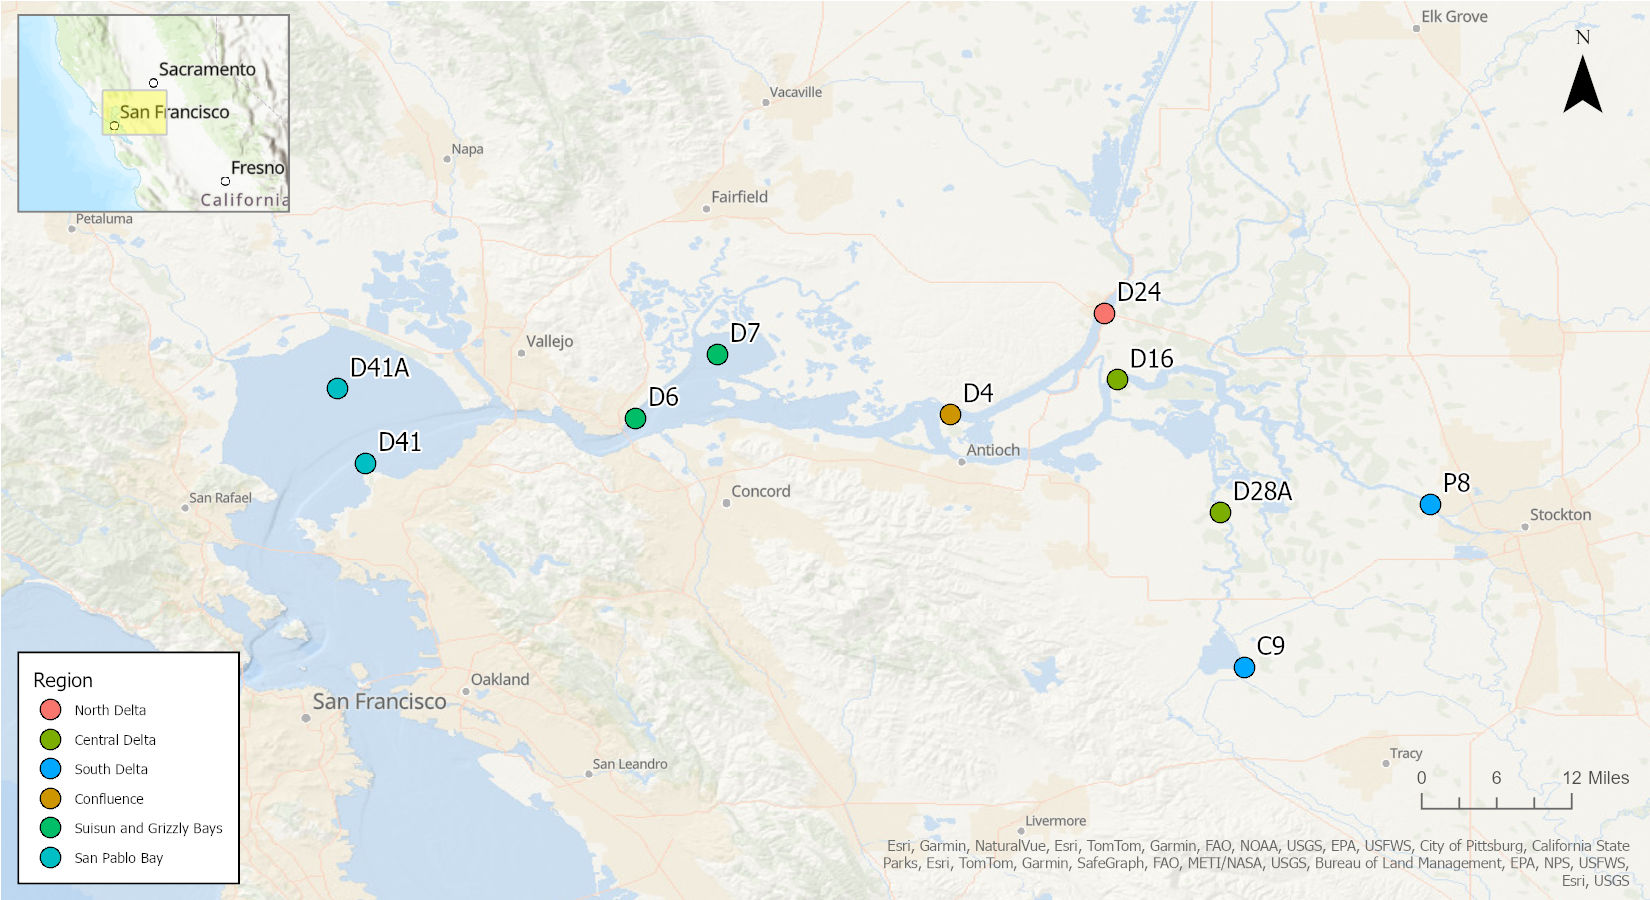
\includegraphics[width=1\linewidth,height=\textheight,keepaspectratio]{admin/figures-tables/benthic/benthic_station_map_pdf.jpg}

}

\caption{\label{fig-stations}Map of EMP's benthic field sites.}

\end{figure}%

\begin{figure}[H]

\centering{

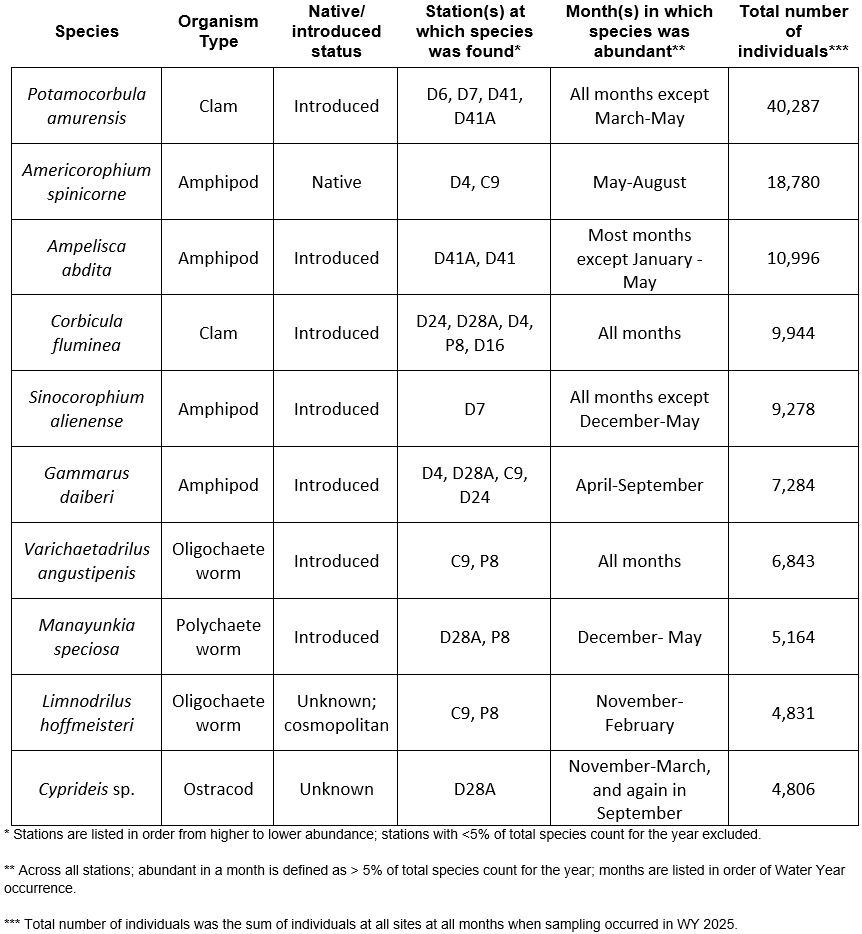
\includegraphics[width=1\linewidth,height=\textheight,keepaspectratio]{admin/figures-tables/benthic/species_list.png}

}

\caption{\label{fig-abund}List of ten most numerous benthic invertebrate
species found at EMP sites.}

\end{figure}%

\begin{figure}[H]

\centering{

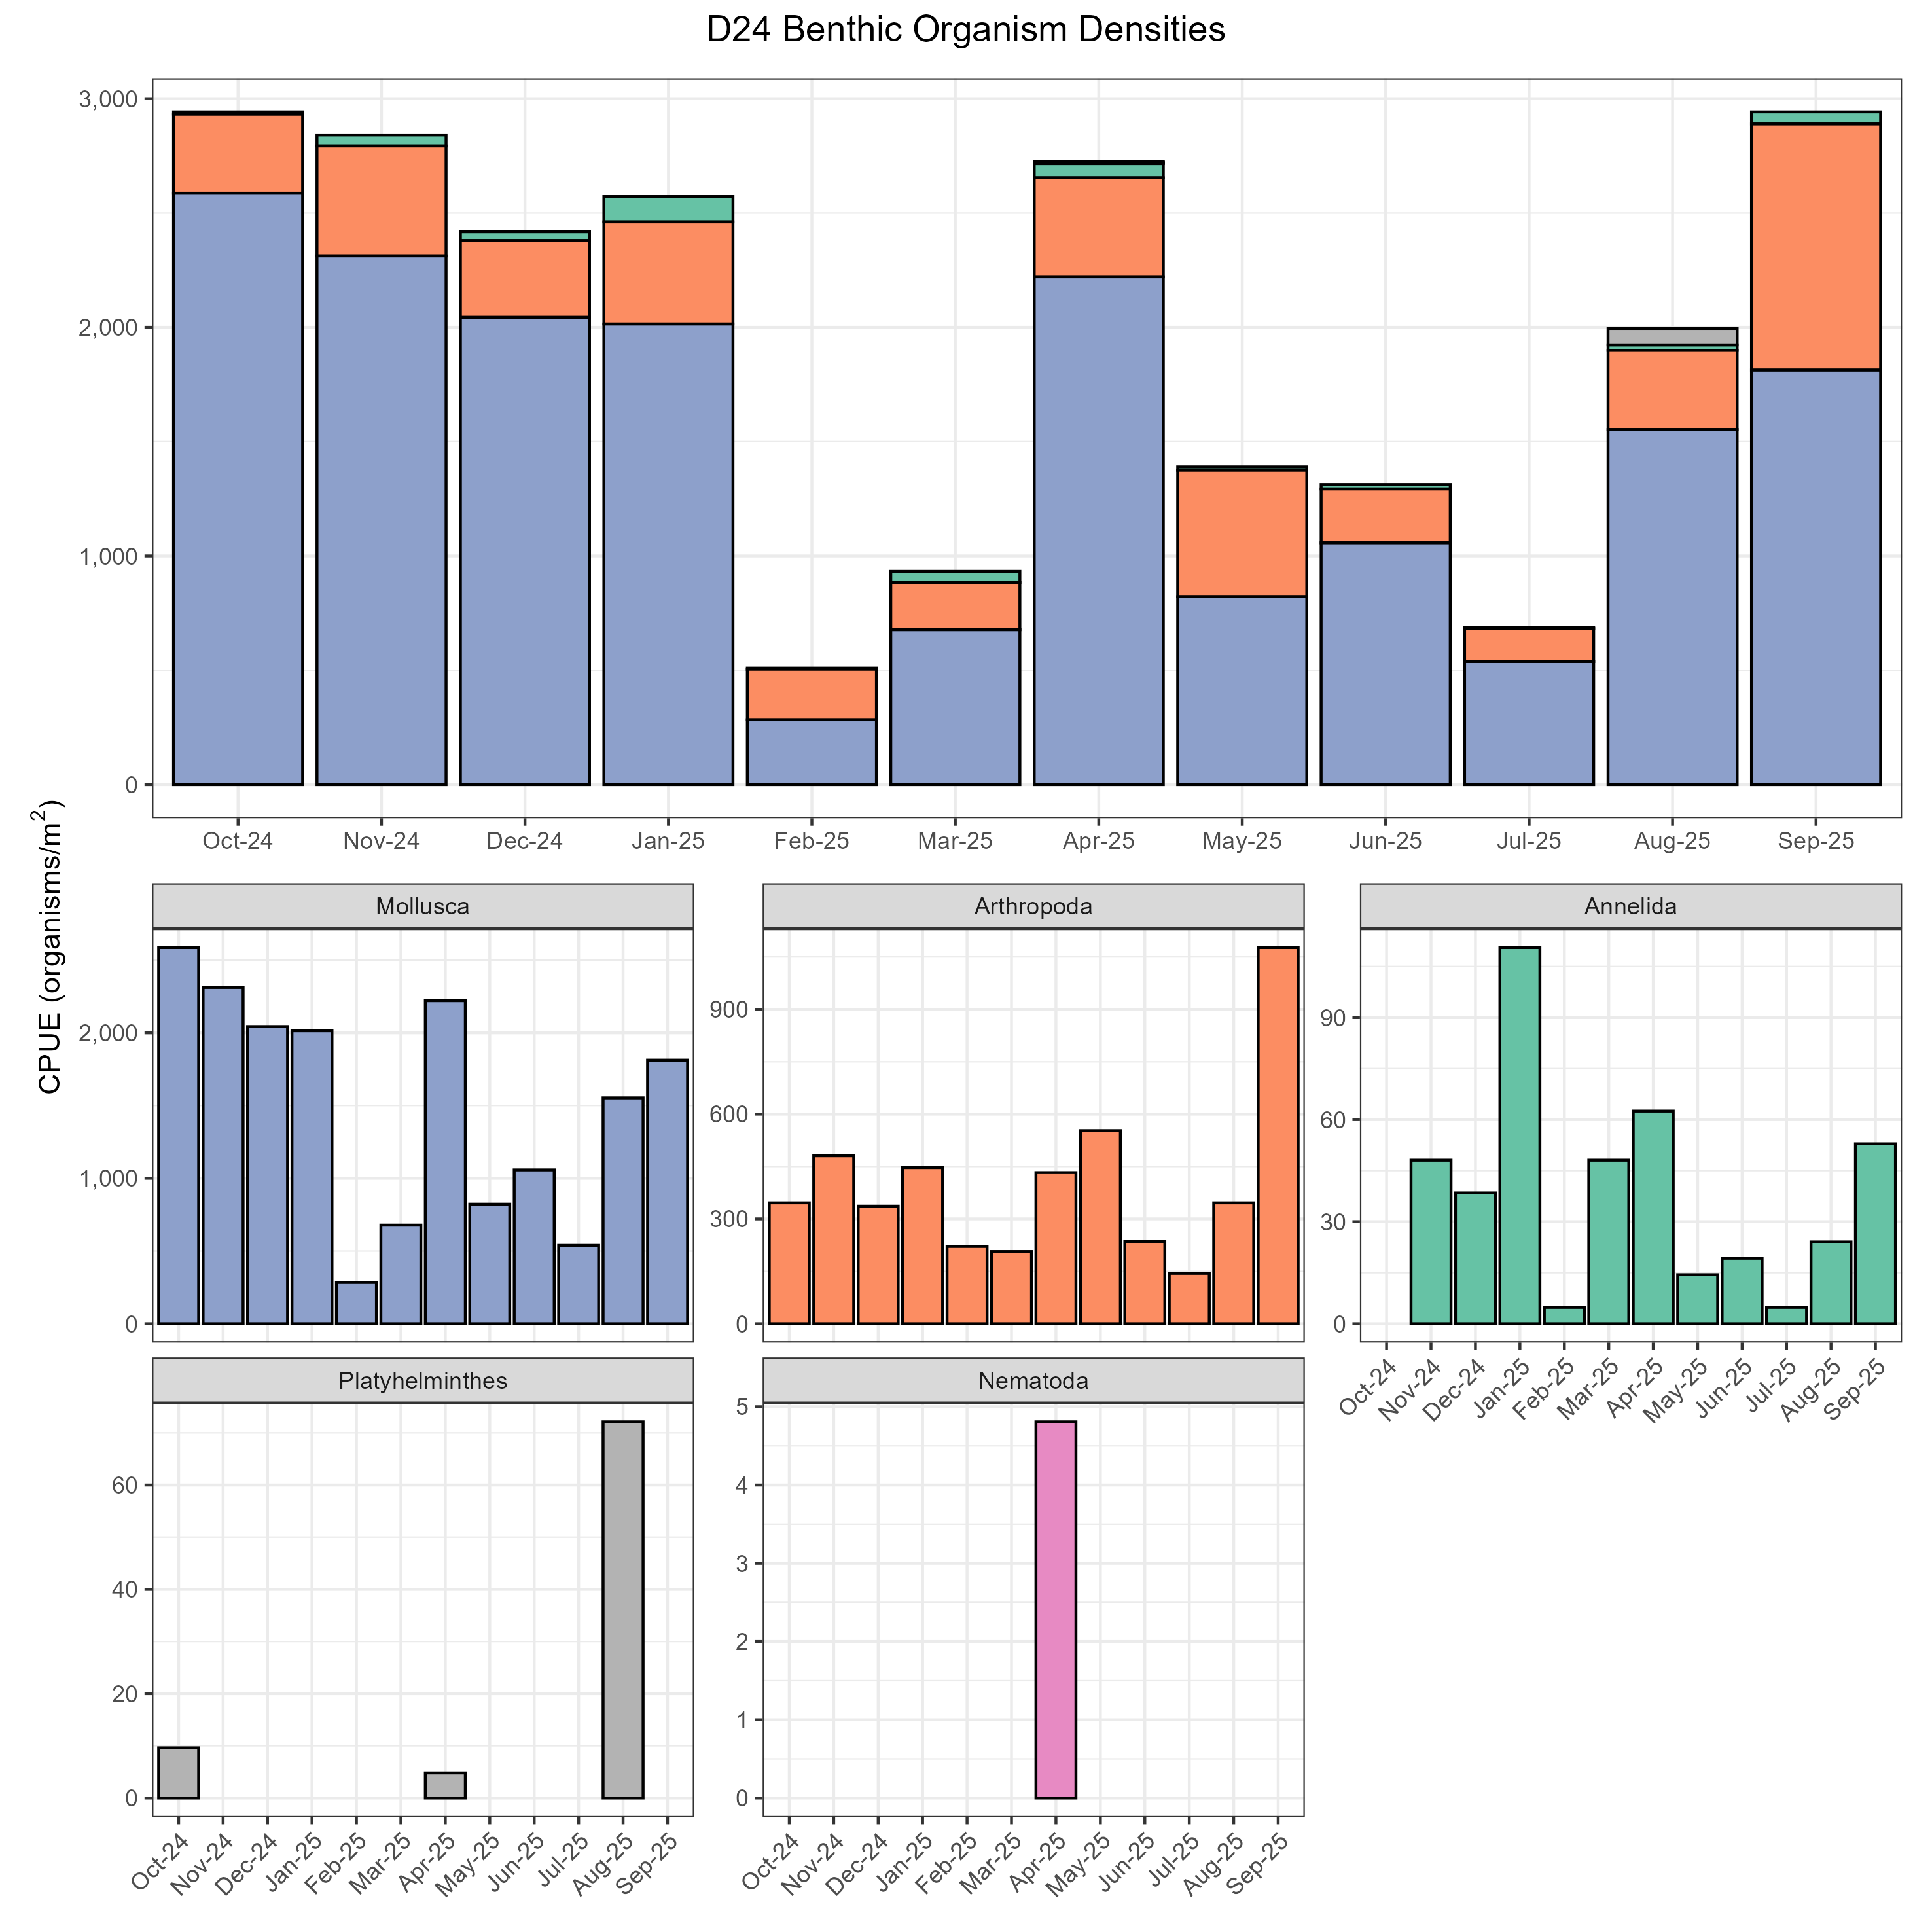
\includegraphics[width=1\linewidth,height=\textheight,keepaspectratio]{admin/figures-tables/benthic/benthic_bar_d24.png}

}

\caption{\label{fig-benthic_d24}Density of benthic organisms, by month,
collected at station D24.}

\end{figure}%

\begin{figure}[H]

\centering{

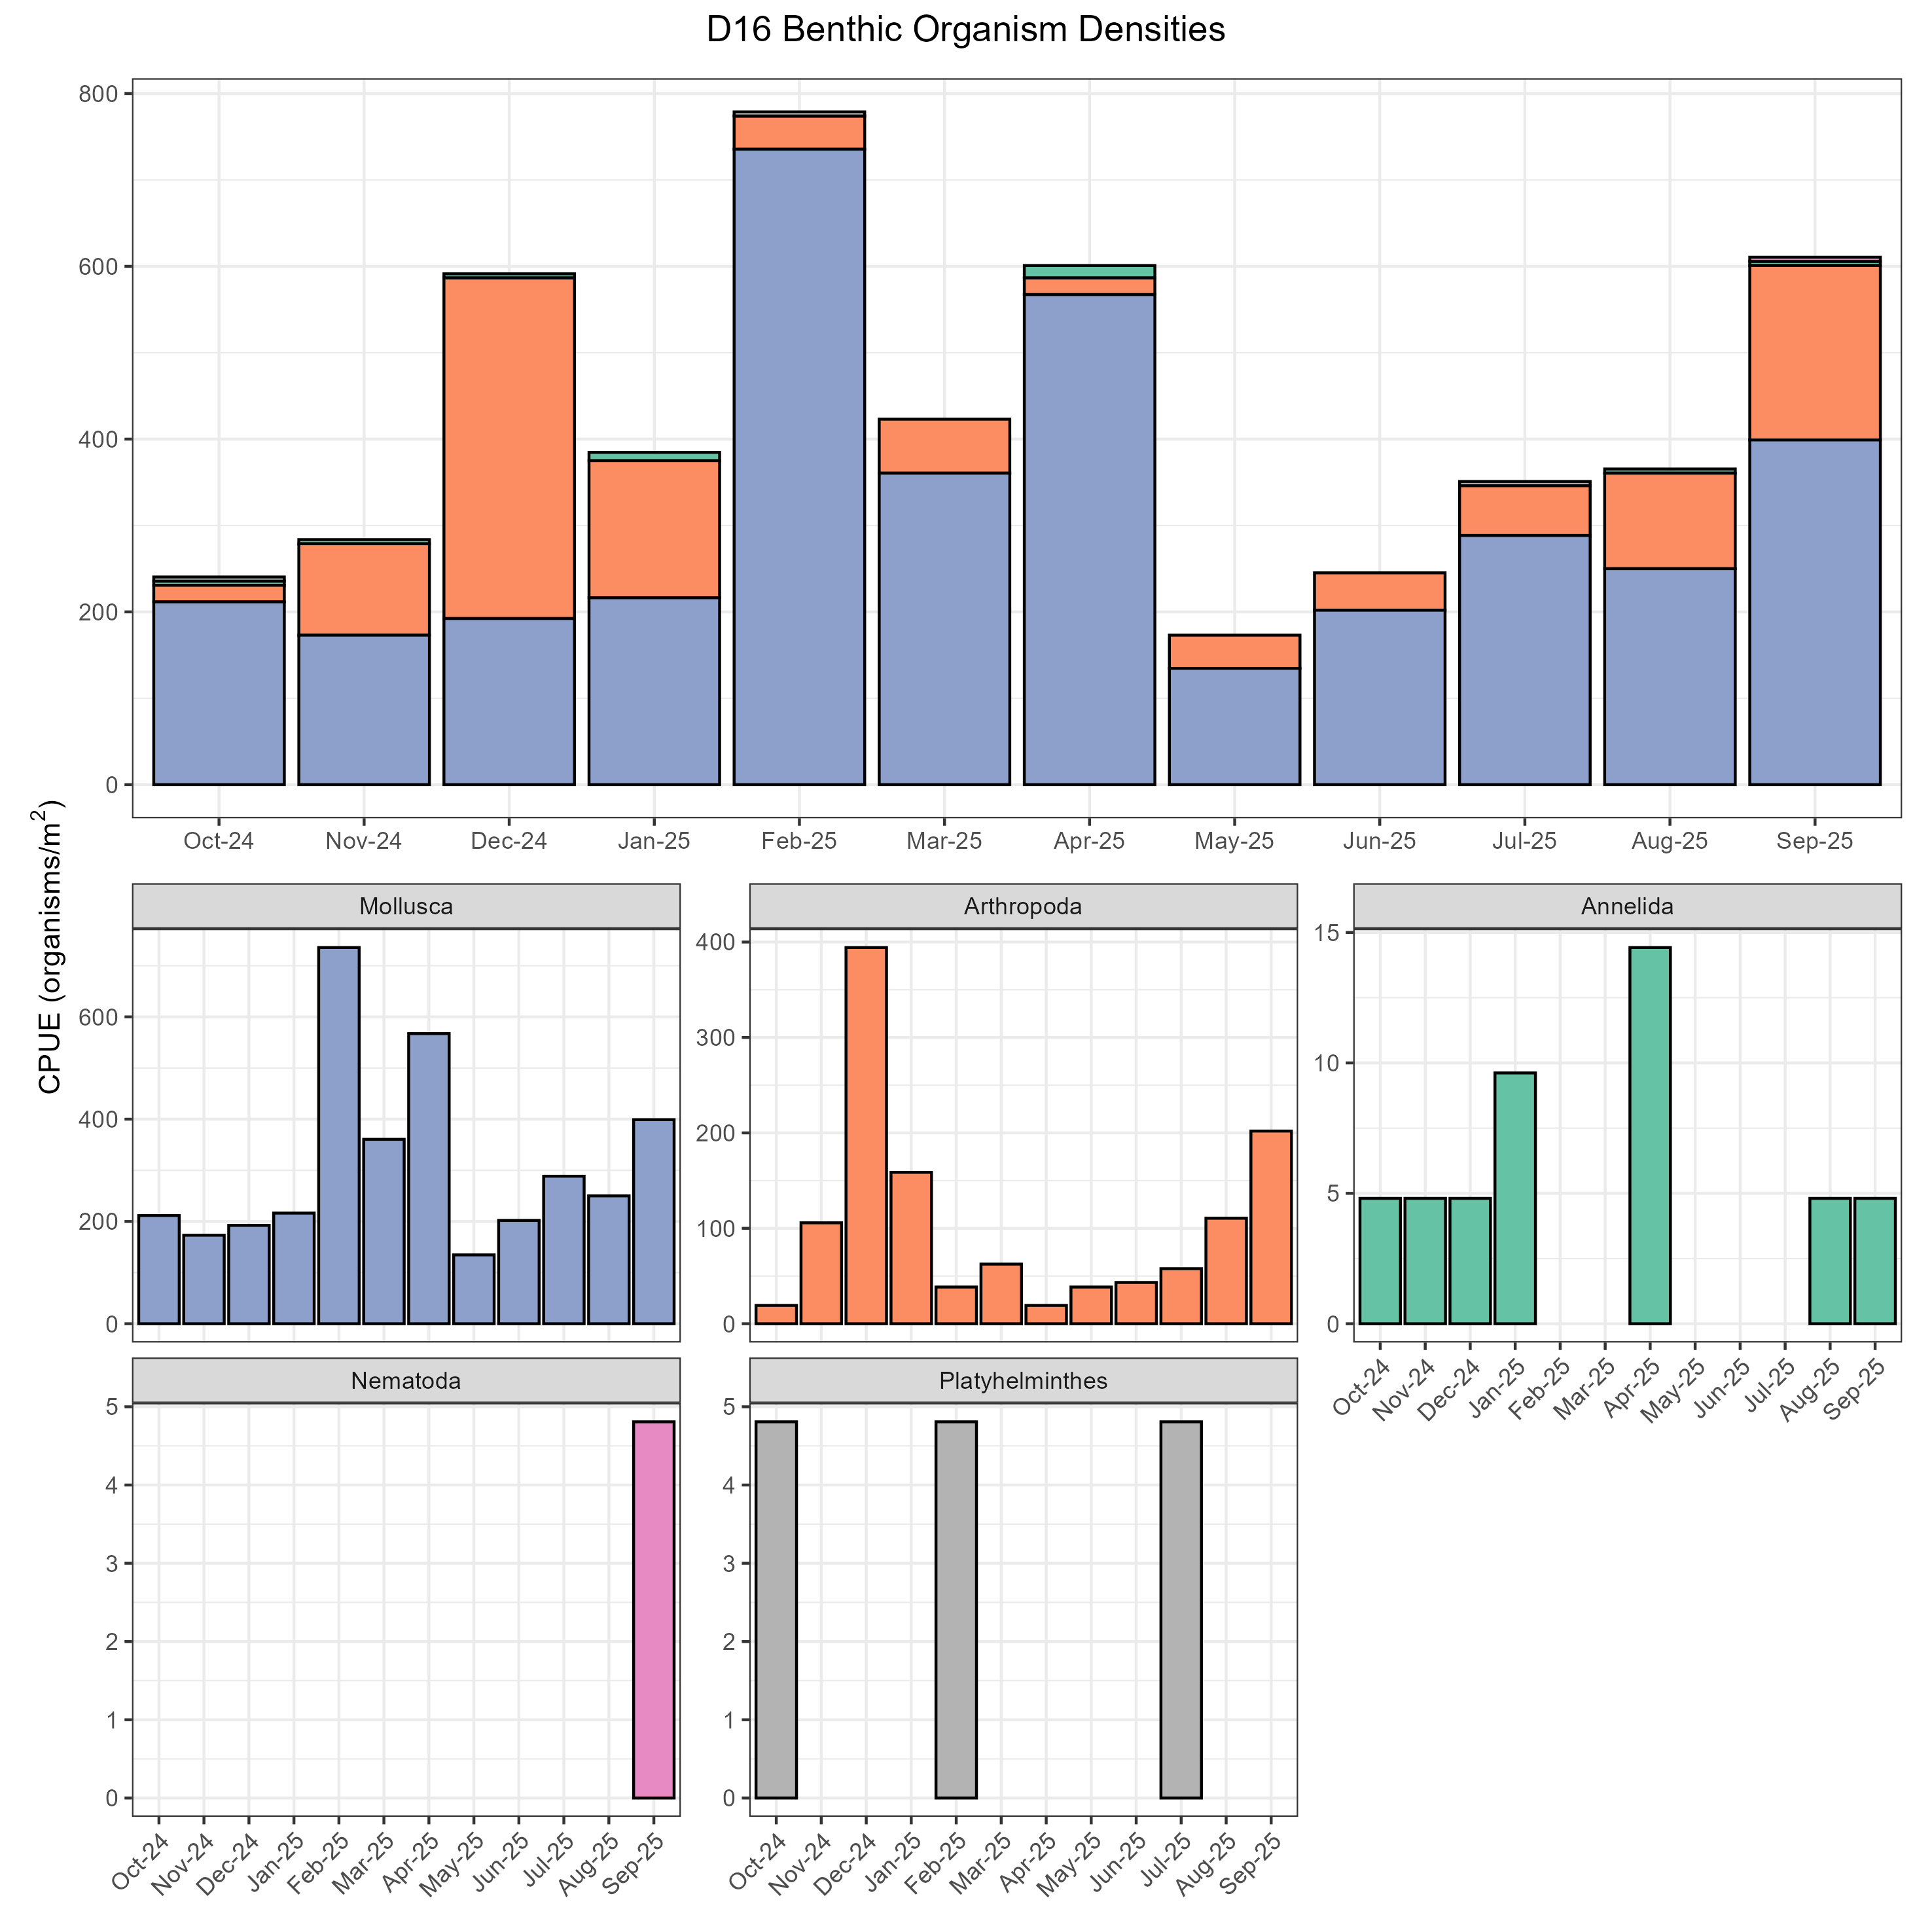
\includegraphics[width=1\linewidth,height=\textheight,keepaspectratio]{admin/figures-tables/benthic/benthic_bar_d16.png}

}

\caption{\label{fig-benthic_d16}Density of benthic organisms, by month,
collected at station D16.}

\end{figure}%

\begin{figure}[H]

\centering{

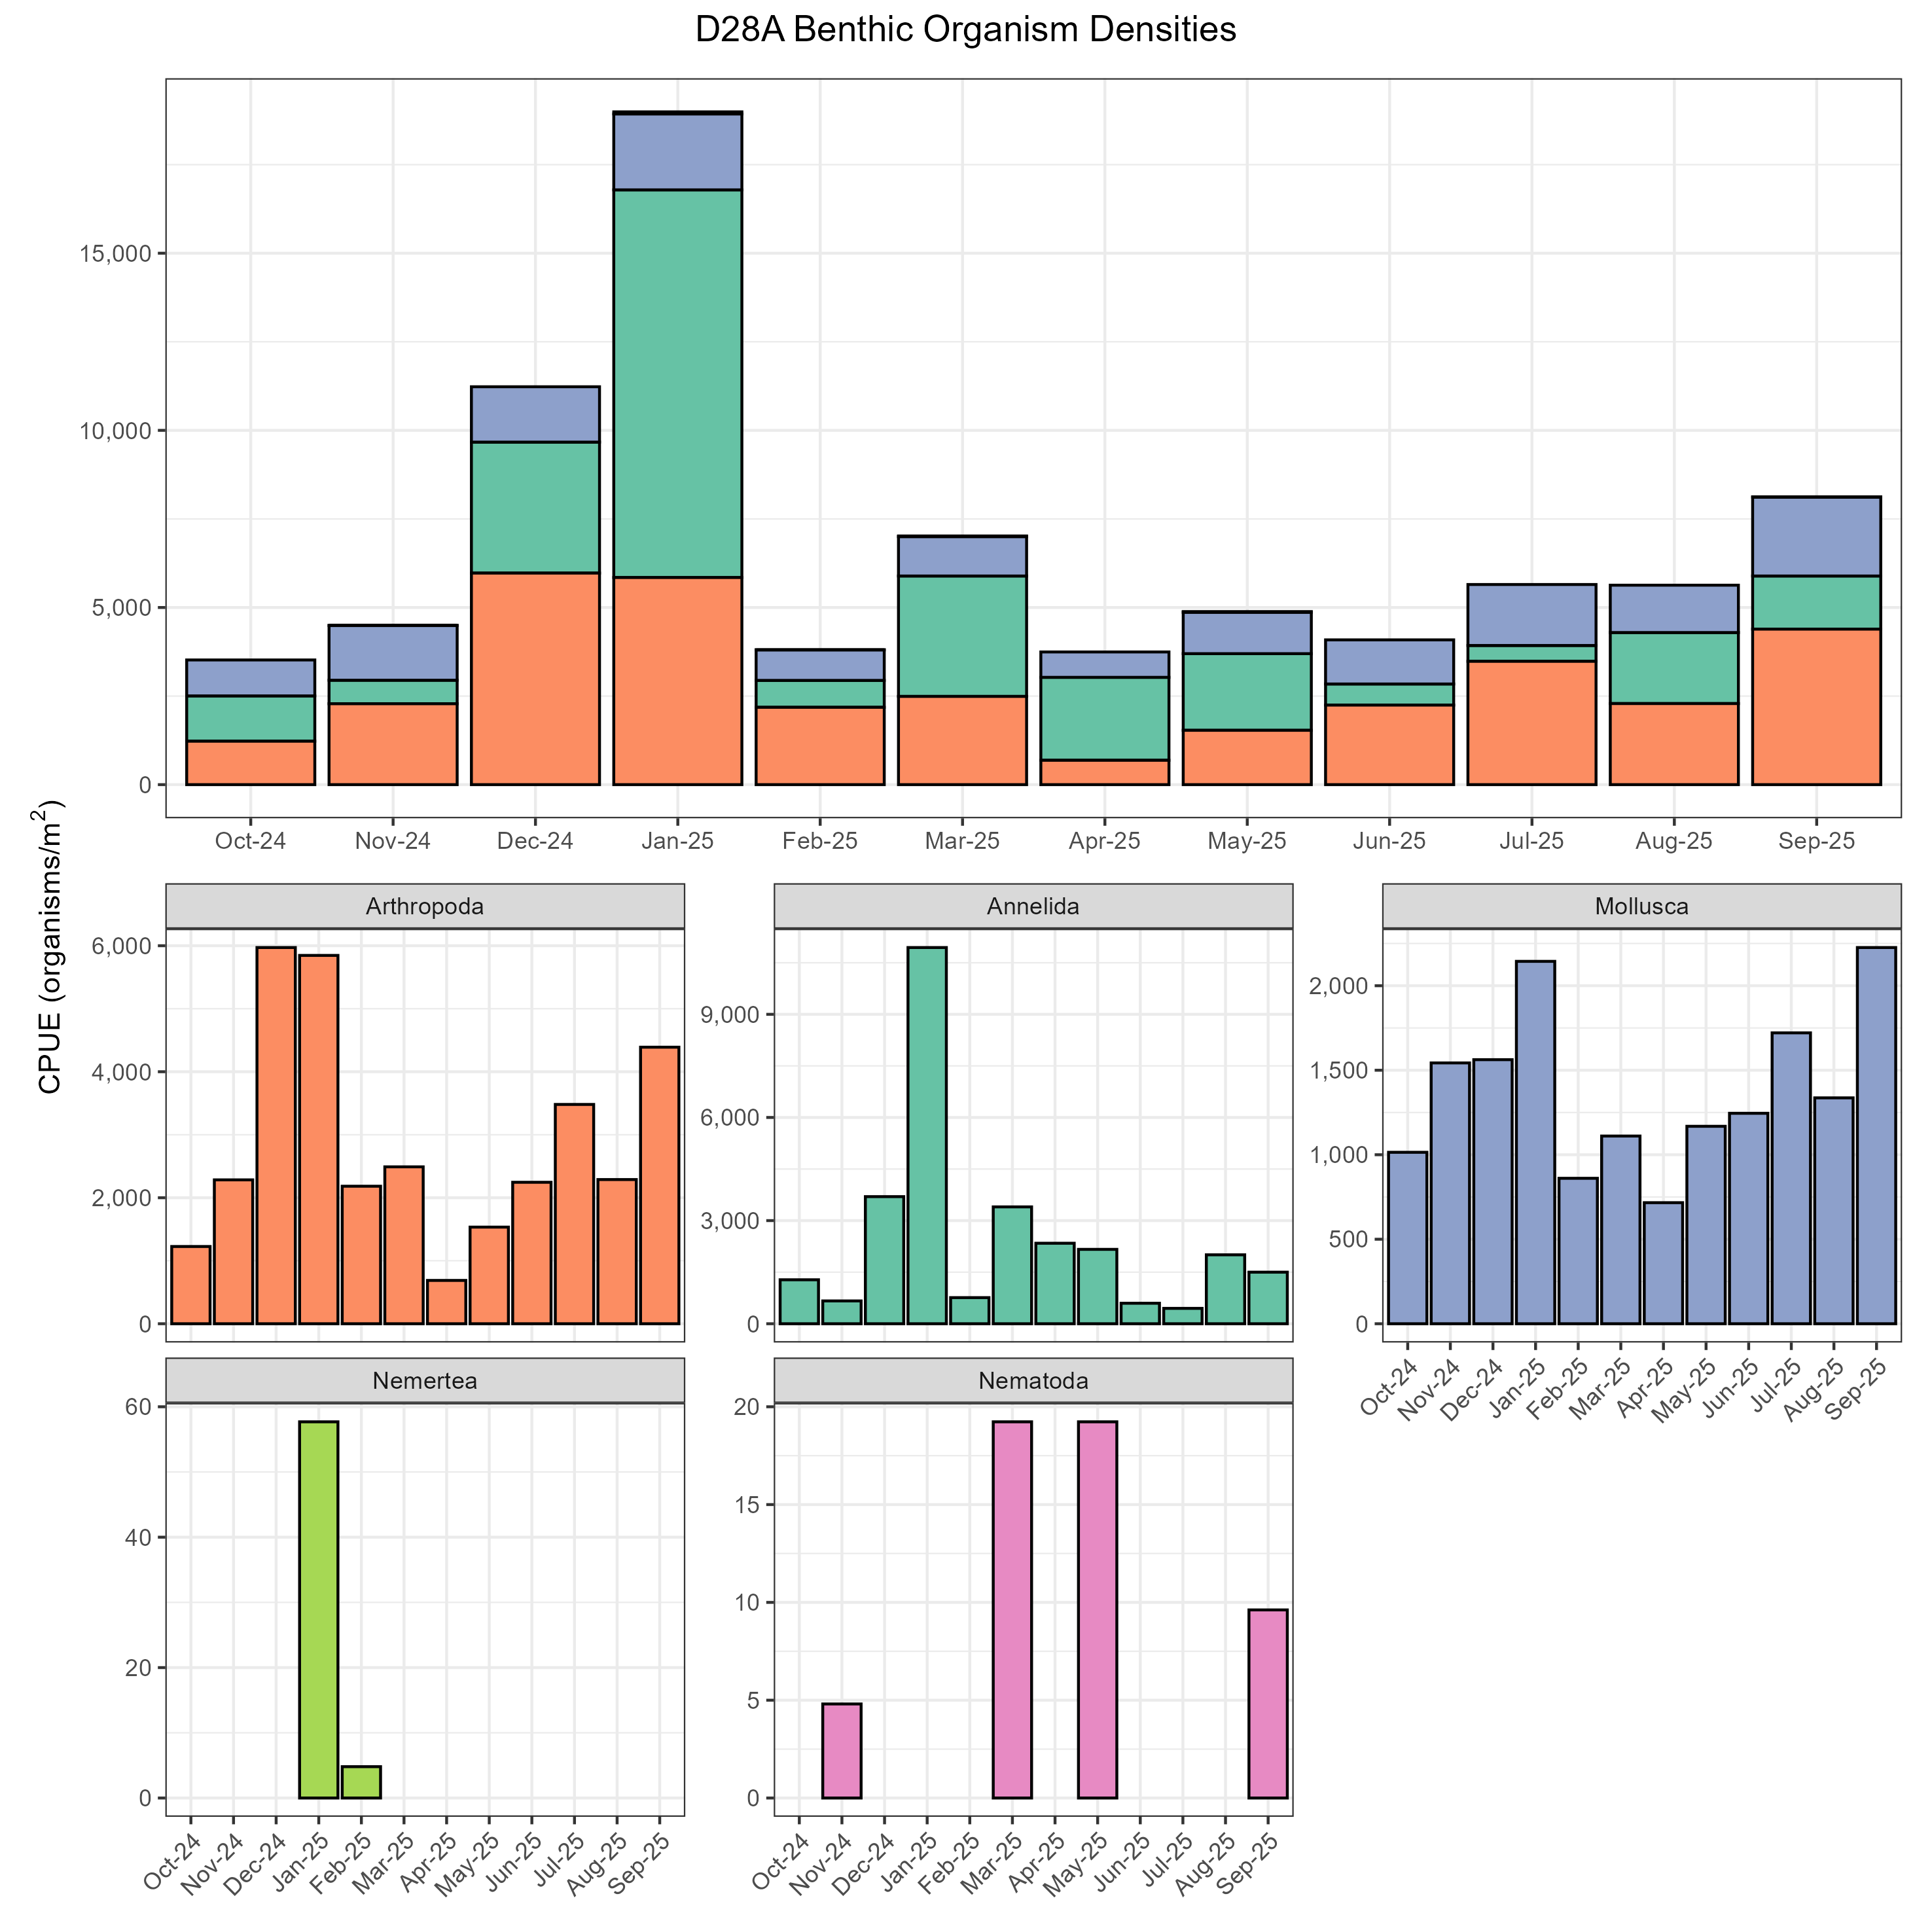
\includegraphics[width=1\linewidth,height=\textheight,keepaspectratio]{admin/figures-tables/benthic/benthic_bar_d28a.png}

}

\caption{\label{fig-benthic_d28a}Density of benthic organisms, by month,
collected at station D28A.}

\end{figure}%

\begin{figure}[H]

\centering{

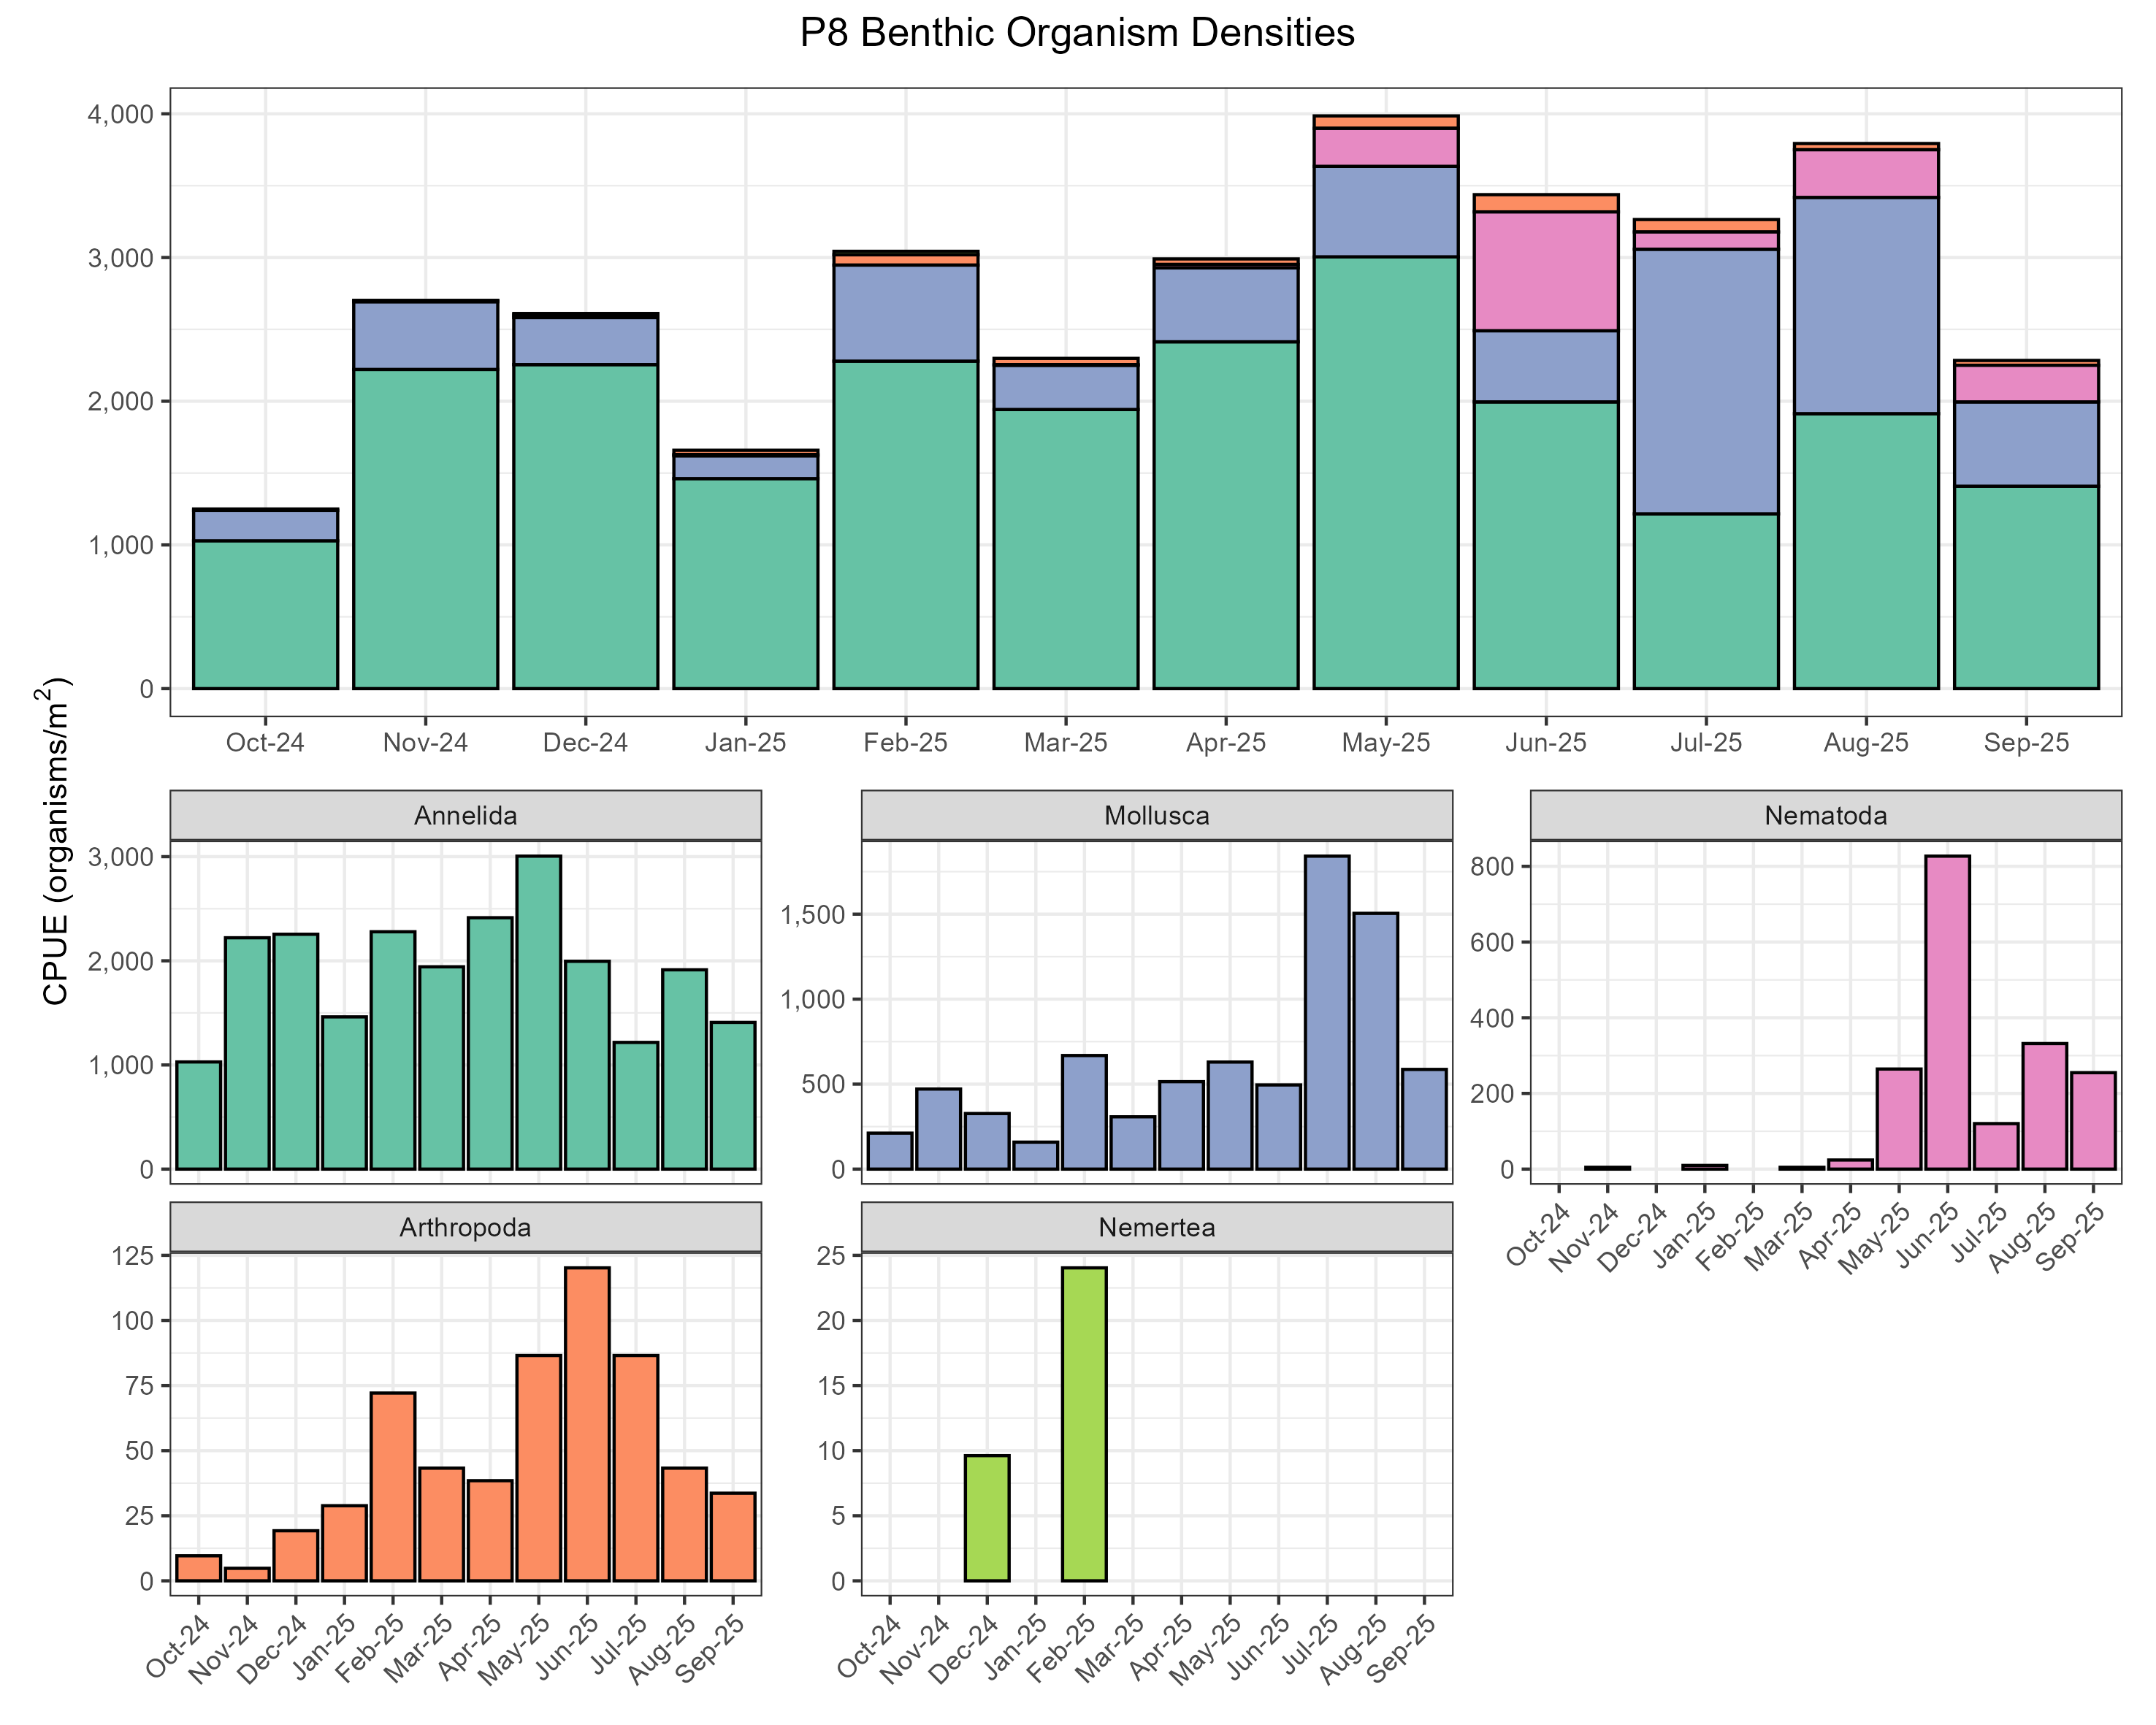
\includegraphics[width=1\linewidth,height=\textheight,keepaspectratio]{admin/figures-tables/benthic/benthic_bar_p8.png}

}

\caption{\label{fig-benthic_p8}Density of benthic organisms, by month,
collected at station P8.}

\end{figure}%

\begin{figure}[H]

\centering{

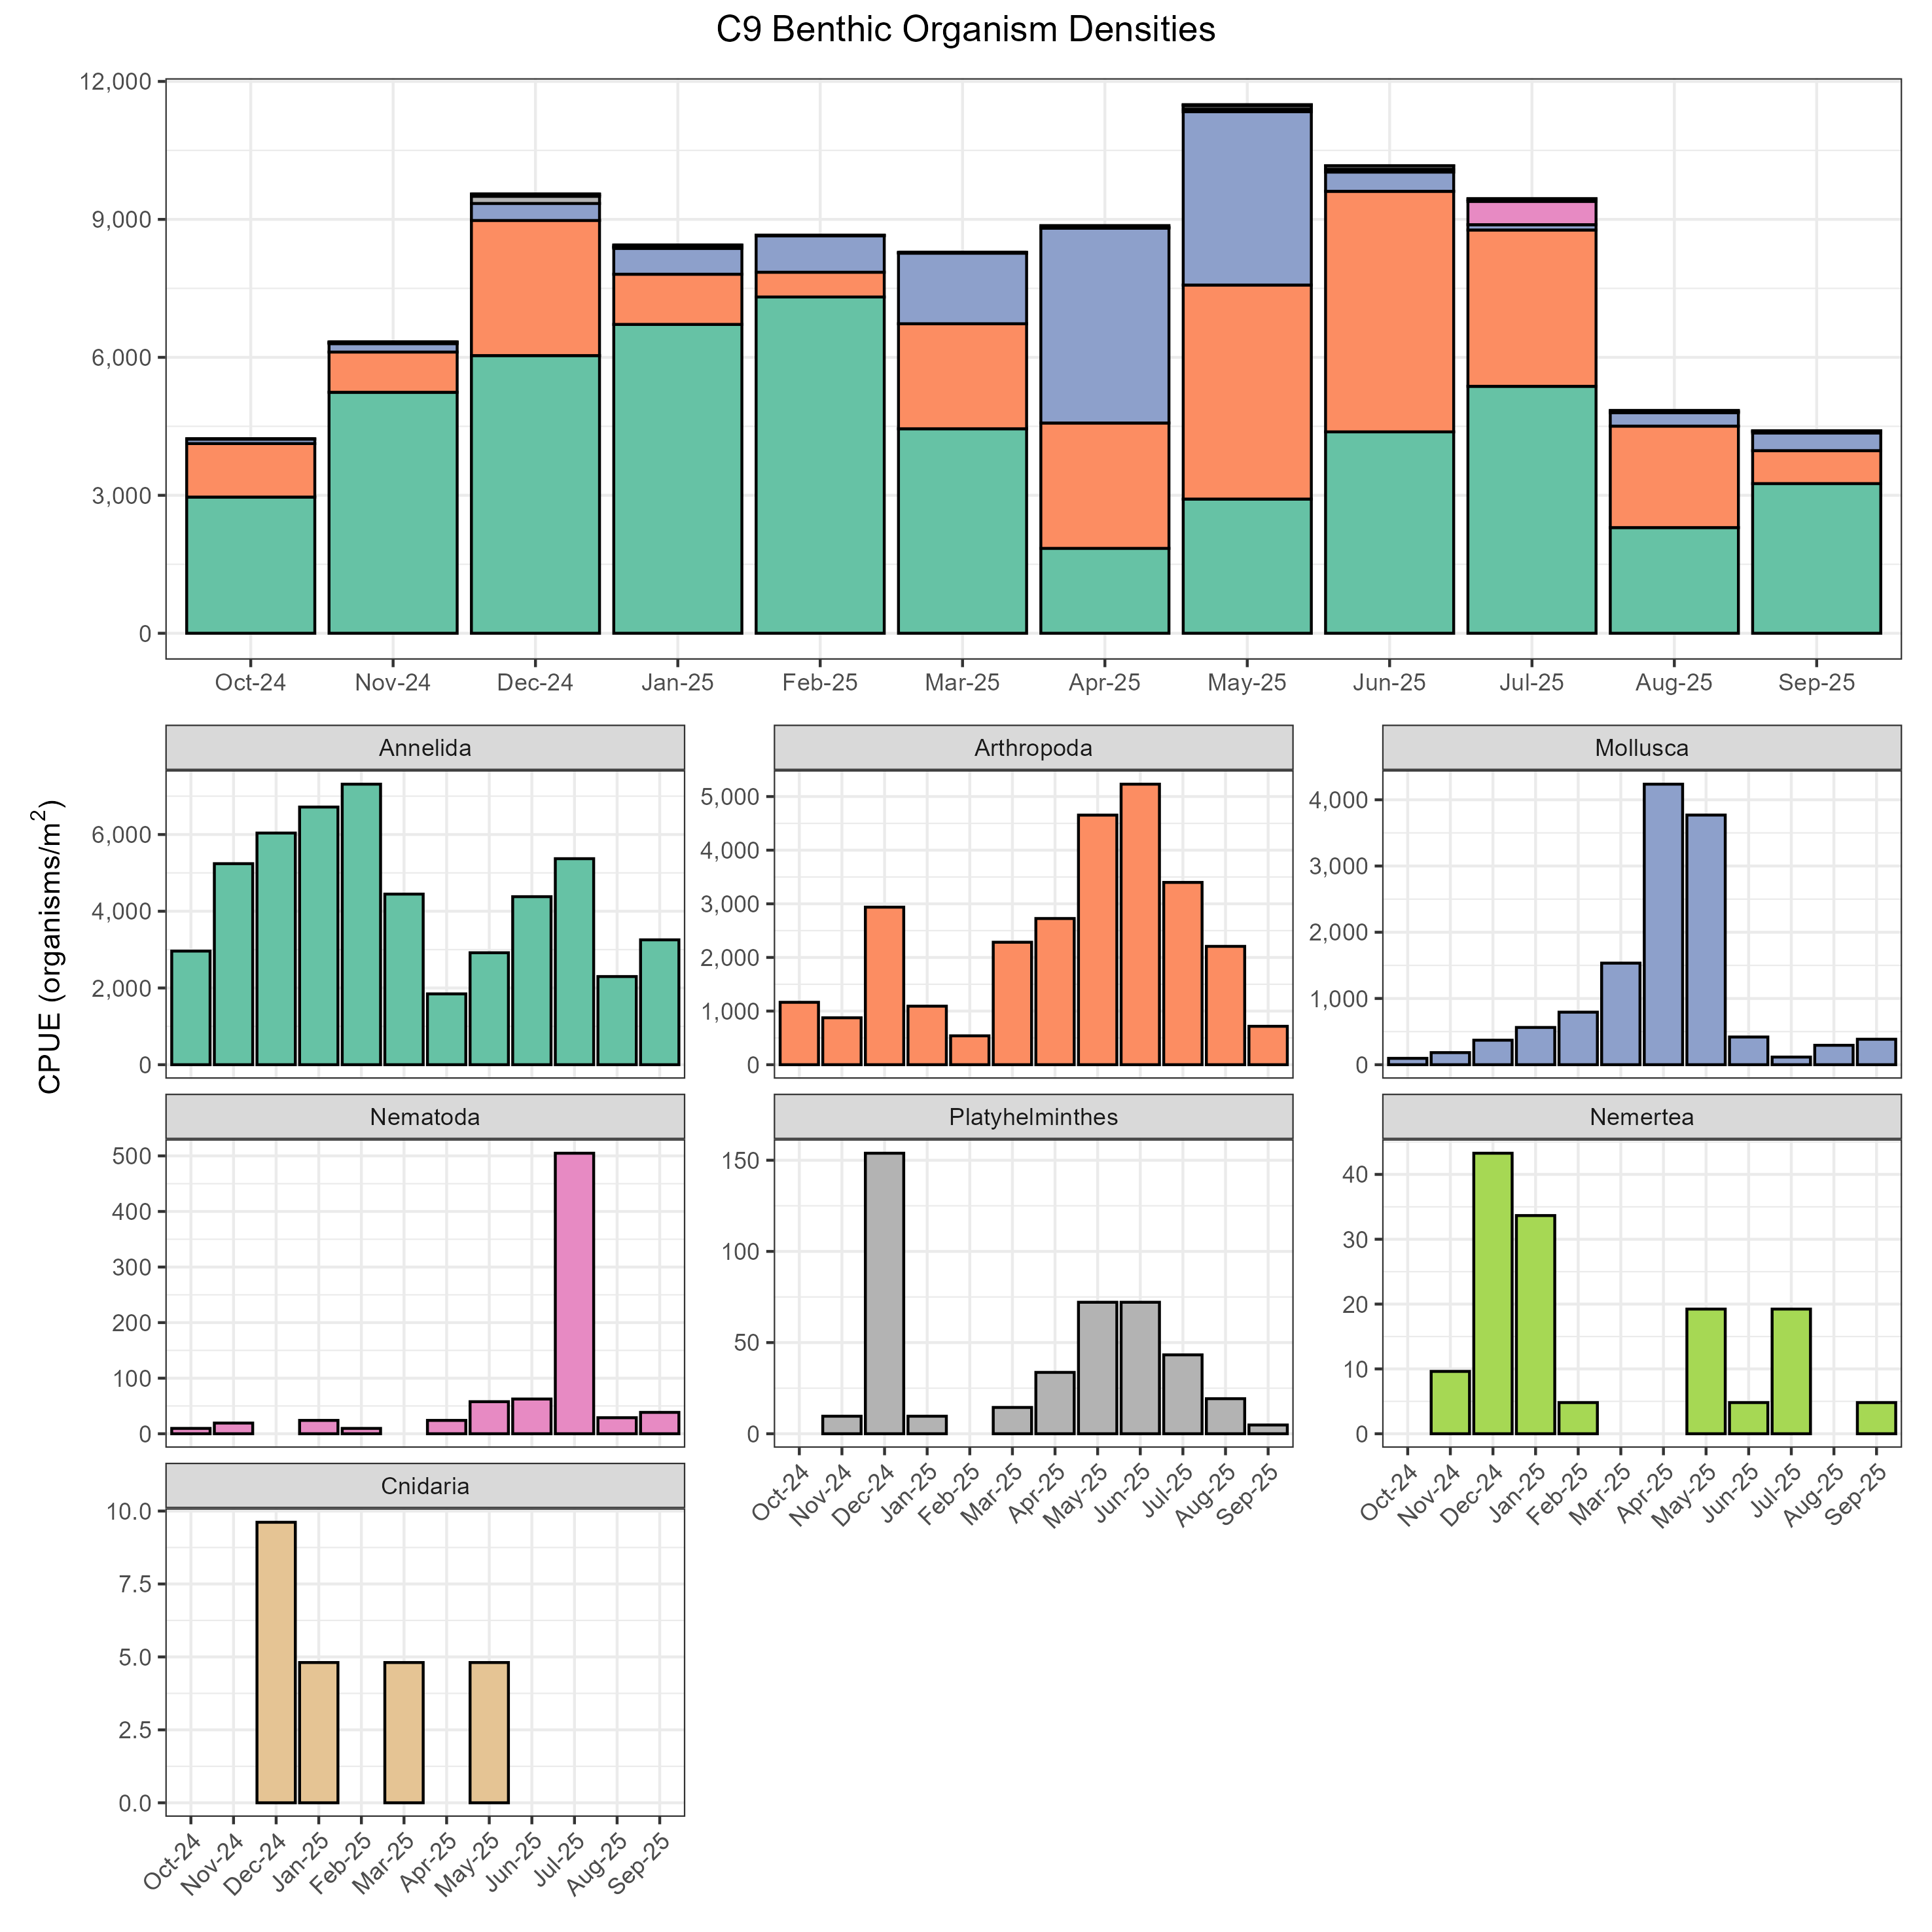
\includegraphics[width=1\linewidth,height=\textheight,keepaspectratio]{admin/figures-tables/benthic/benthic_bar_c9.png}

}

\caption{\label{fig-benthic_c9}Density of benthic organisms, by month,
collected at station C9.}

\end{figure}%

\begin{figure}[H]

\centering{

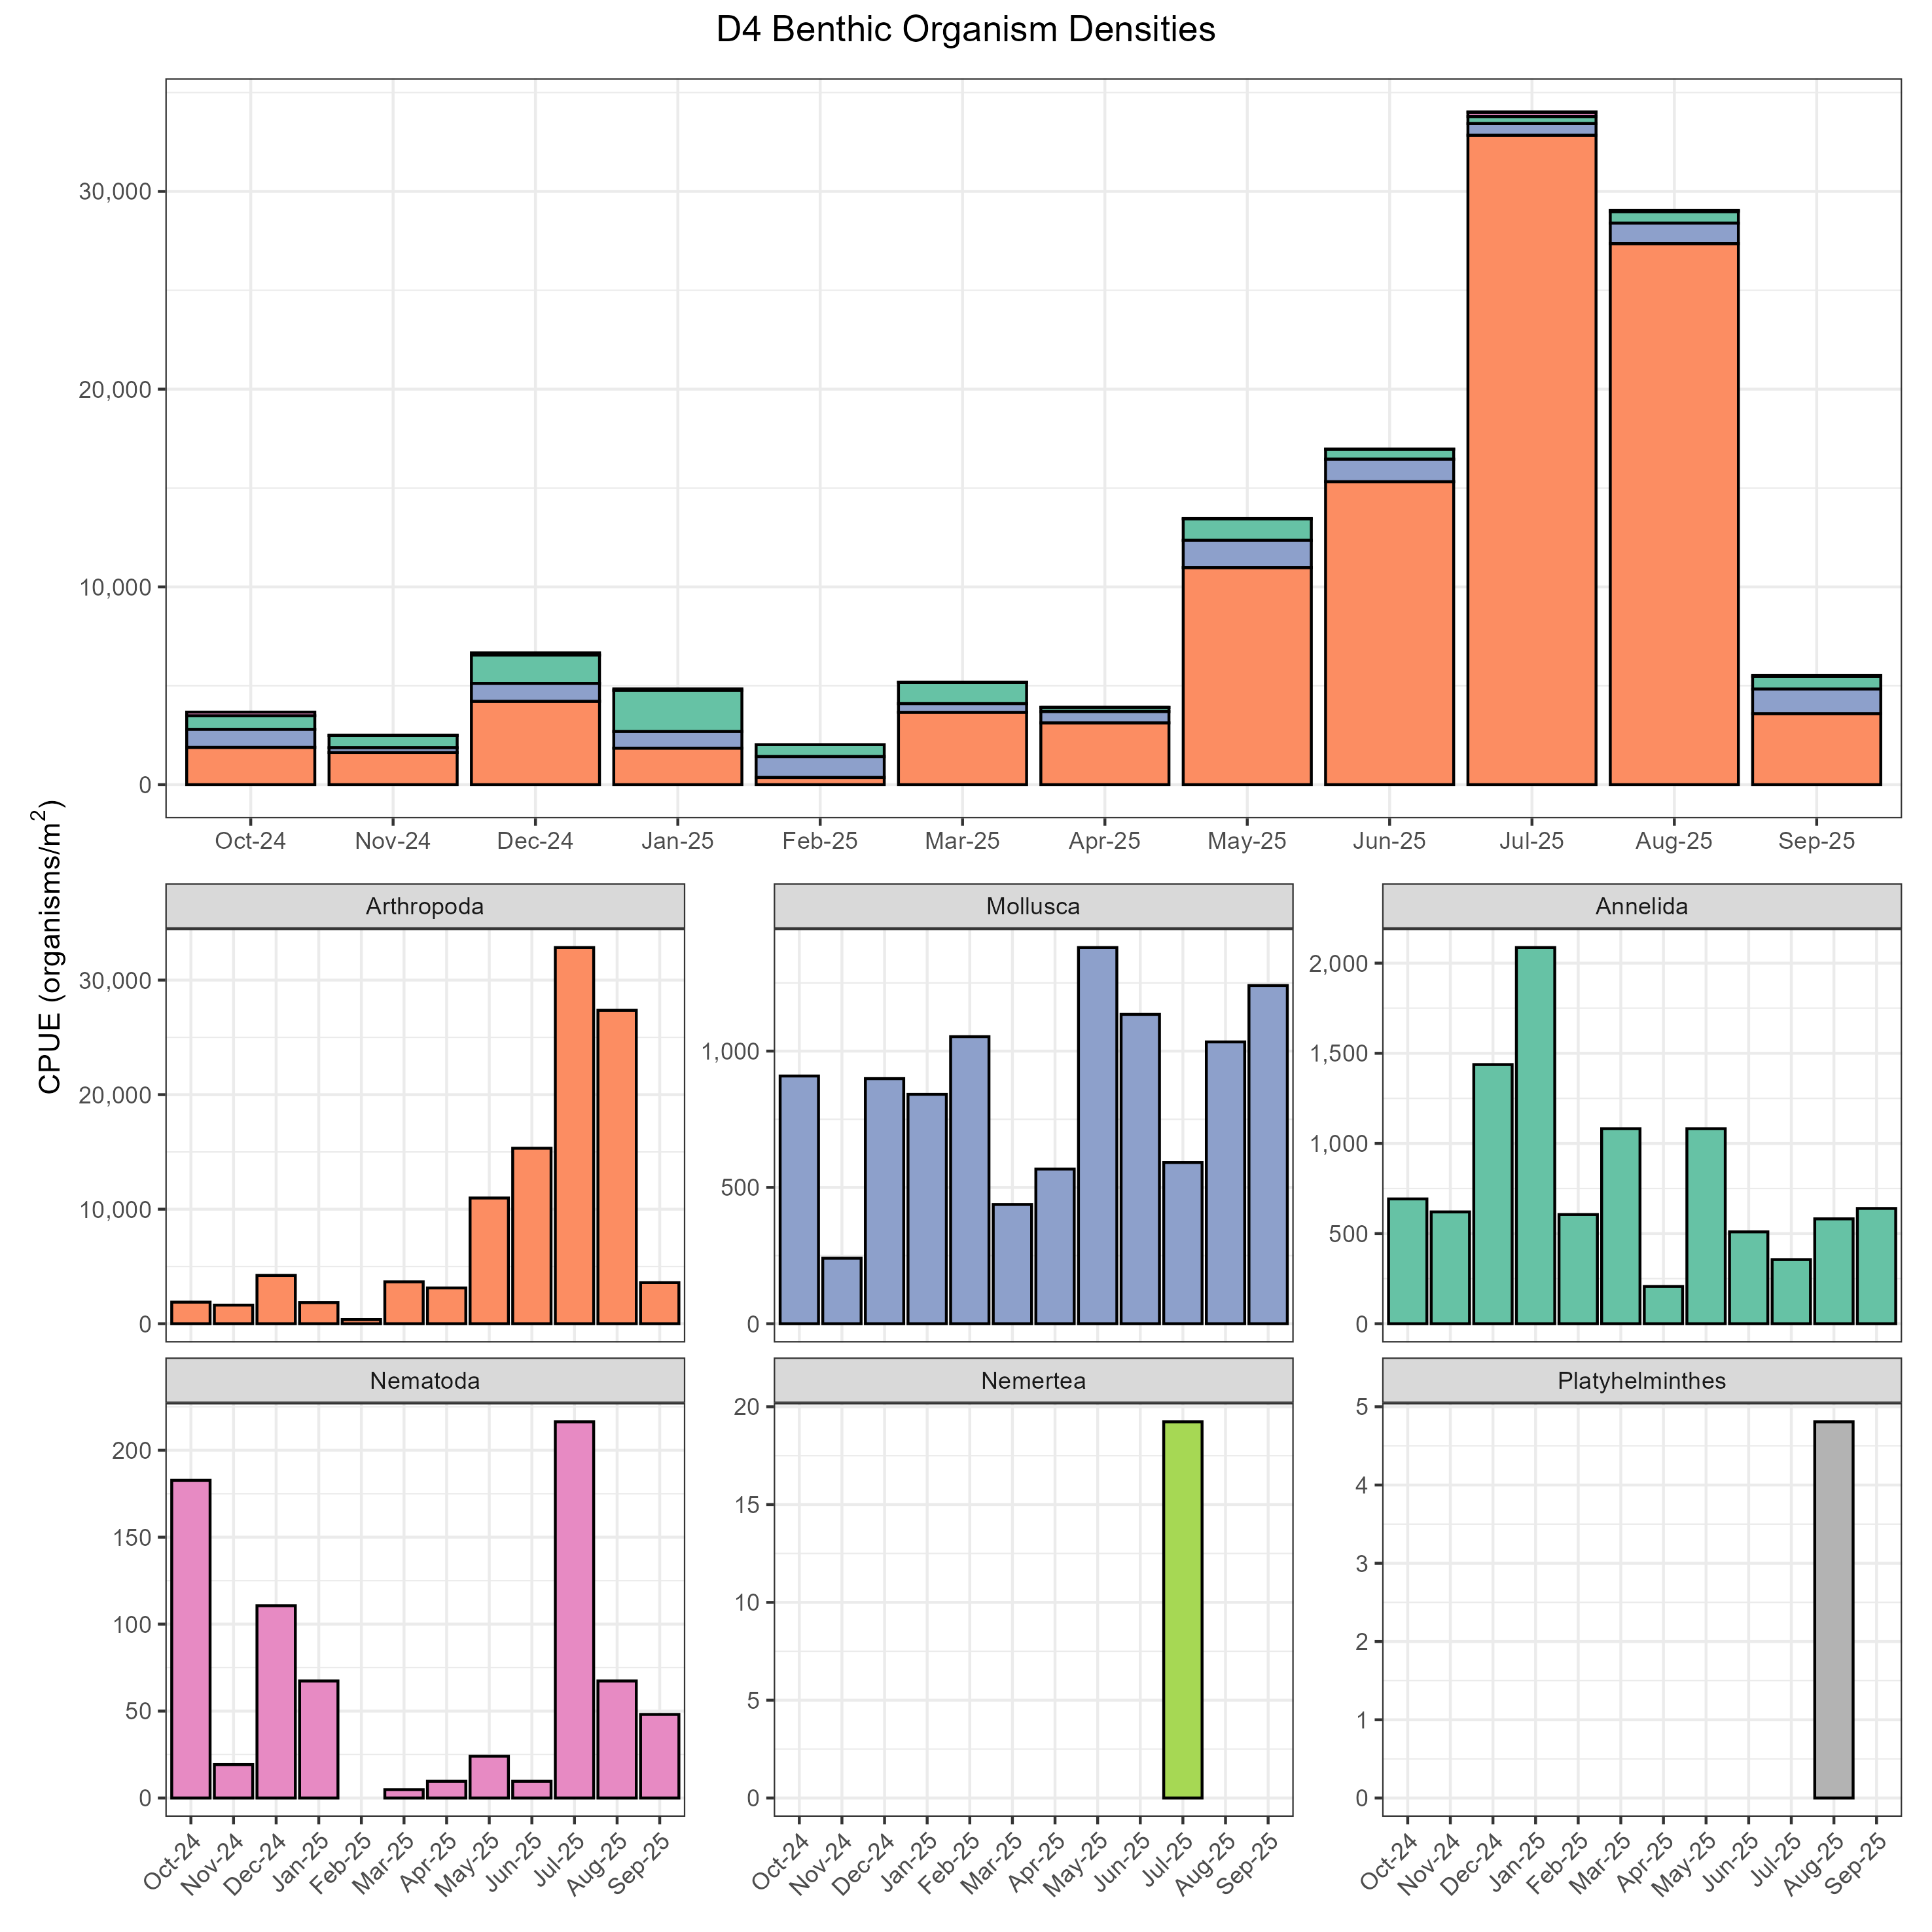
\includegraphics[width=1\linewidth,height=\textheight,keepaspectratio]{admin/figures-tables/benthic/benthic_bar_d4.png}

}

\caption{\label{fig-benthic_d4}Density of benthic organisms, by month,
collected at station D4.}

\end{figure}%

\begin{figure}[H]

\centering{

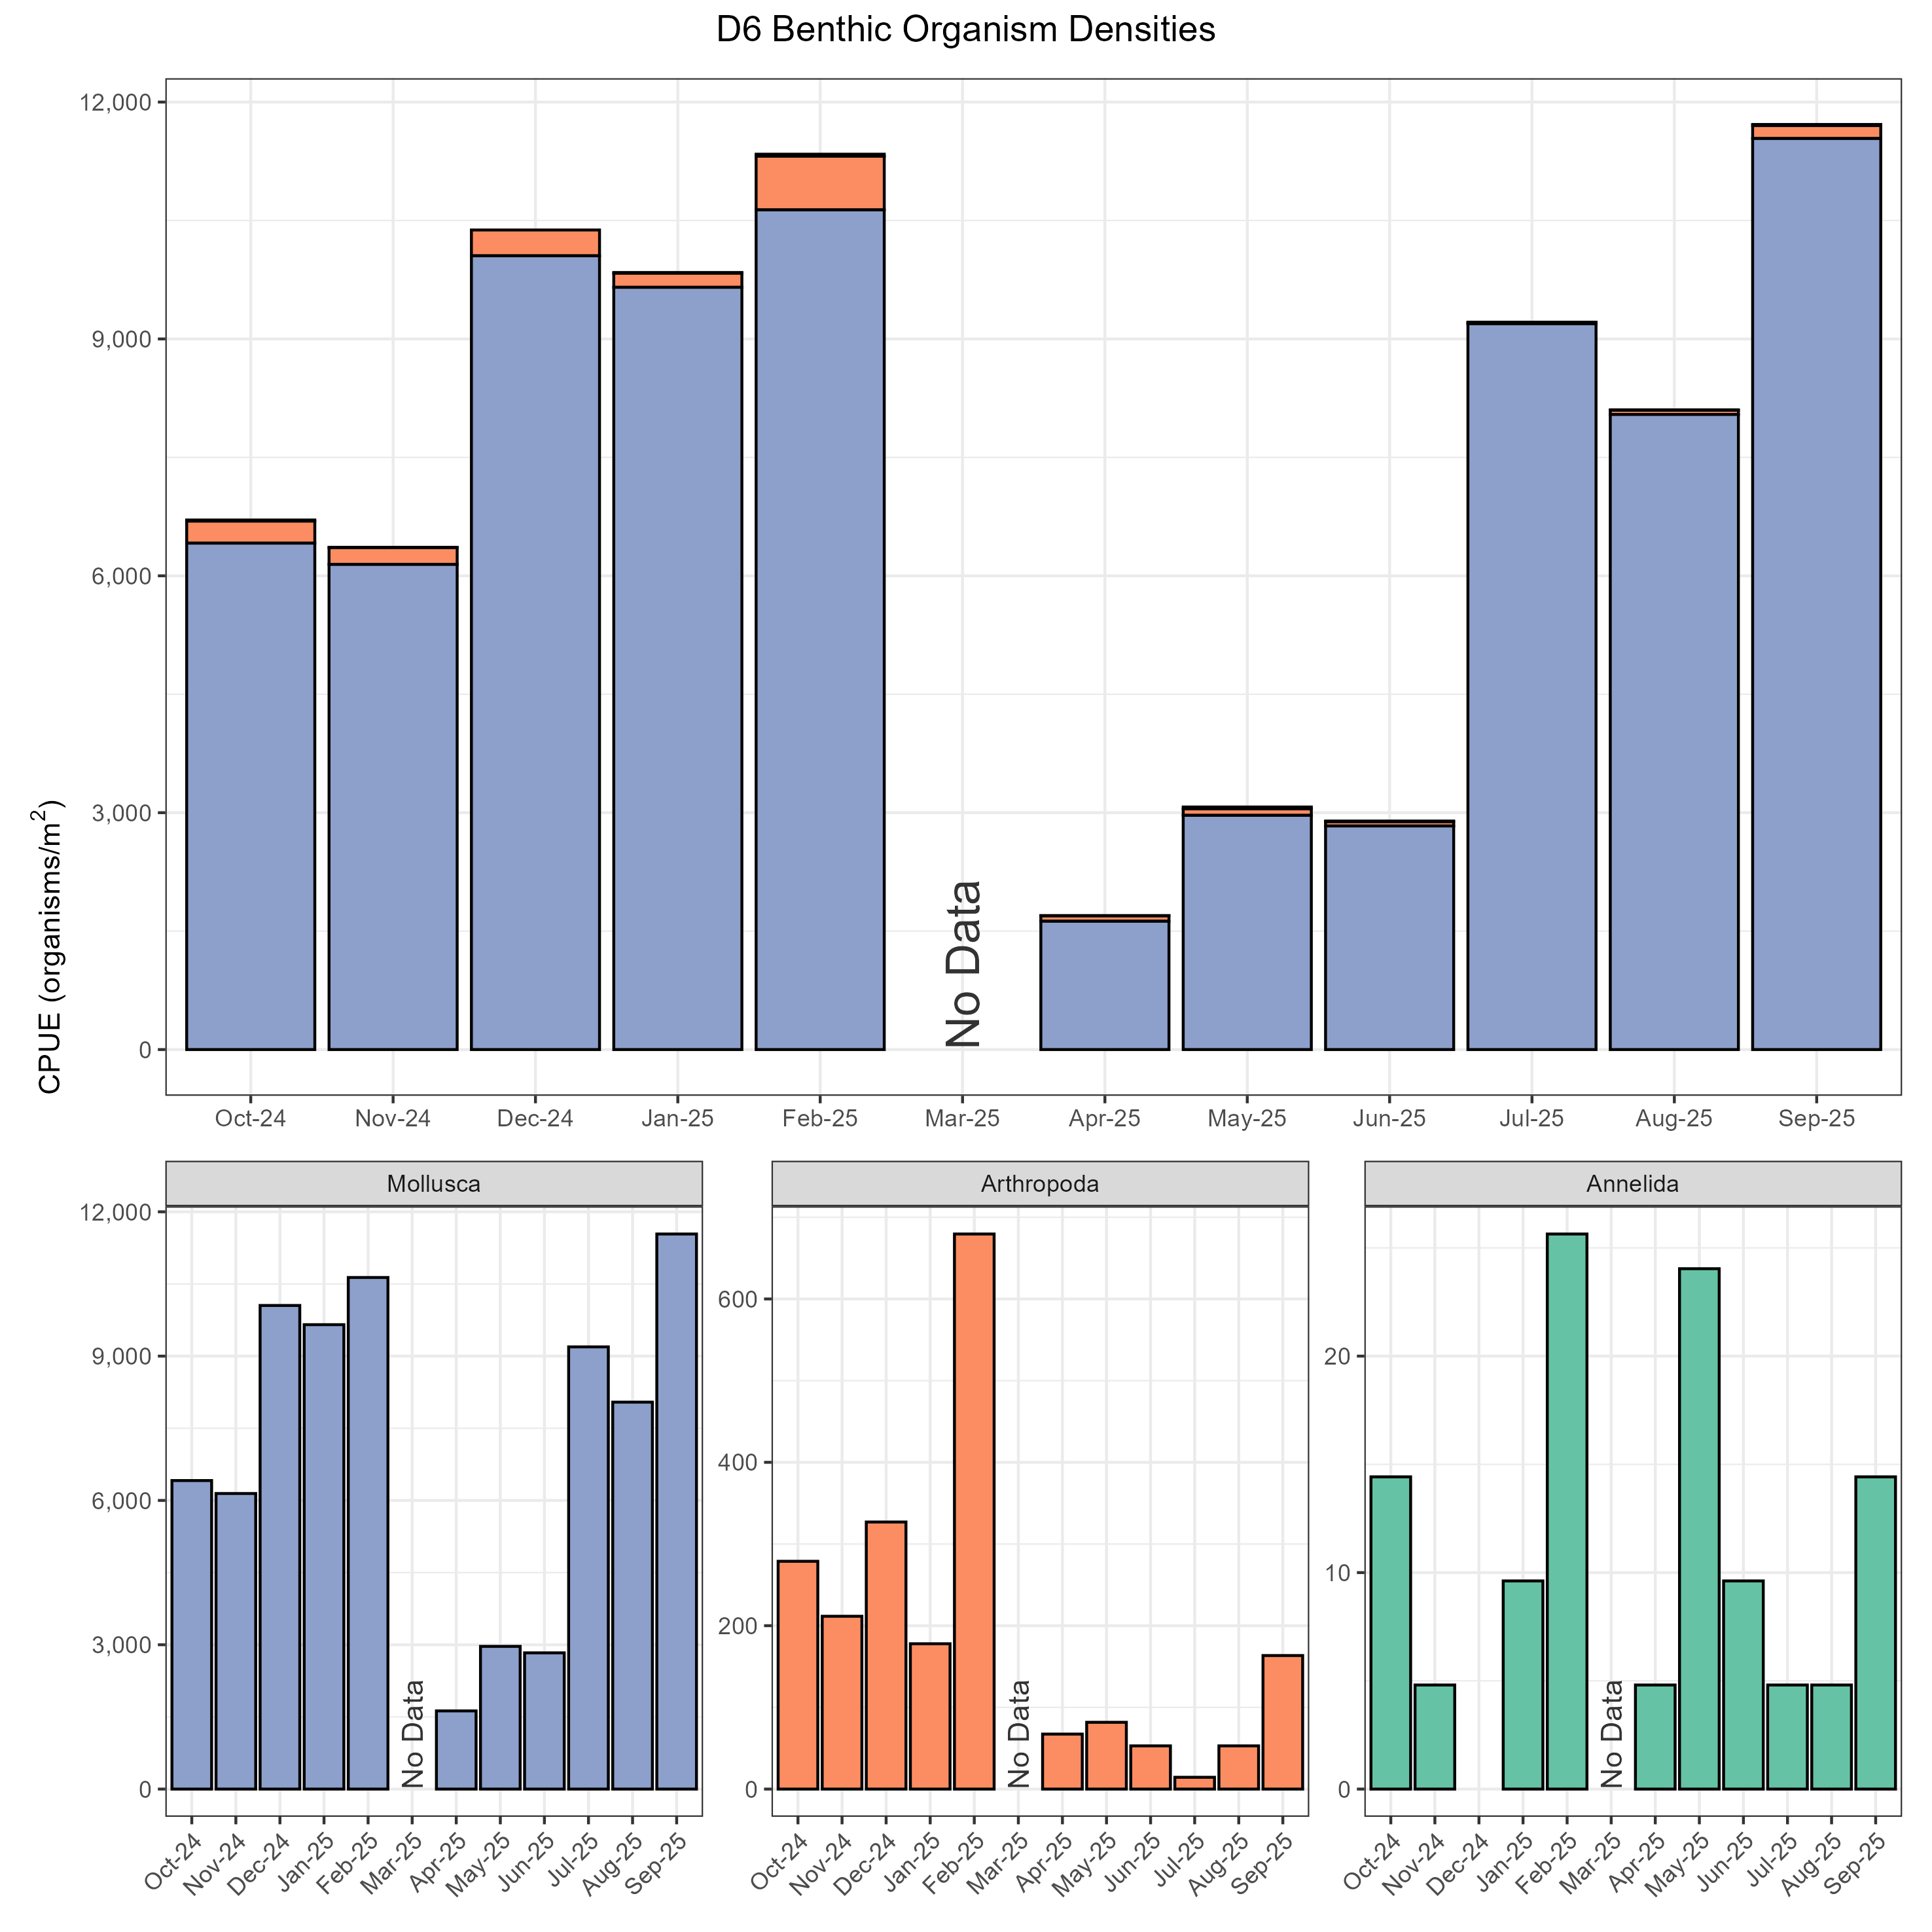
\includegraphics[width=1\linewidth,height=\textheight,keepaspectratio]{admin/figures-tables/benthic/benthic_bar_d6.png}

}

\caption{\label{fig-benthic_d6}Density of benthic organisms, by month,
collected at station D6.}

\end{figure}%

\begin{figure}[H]

\centering{

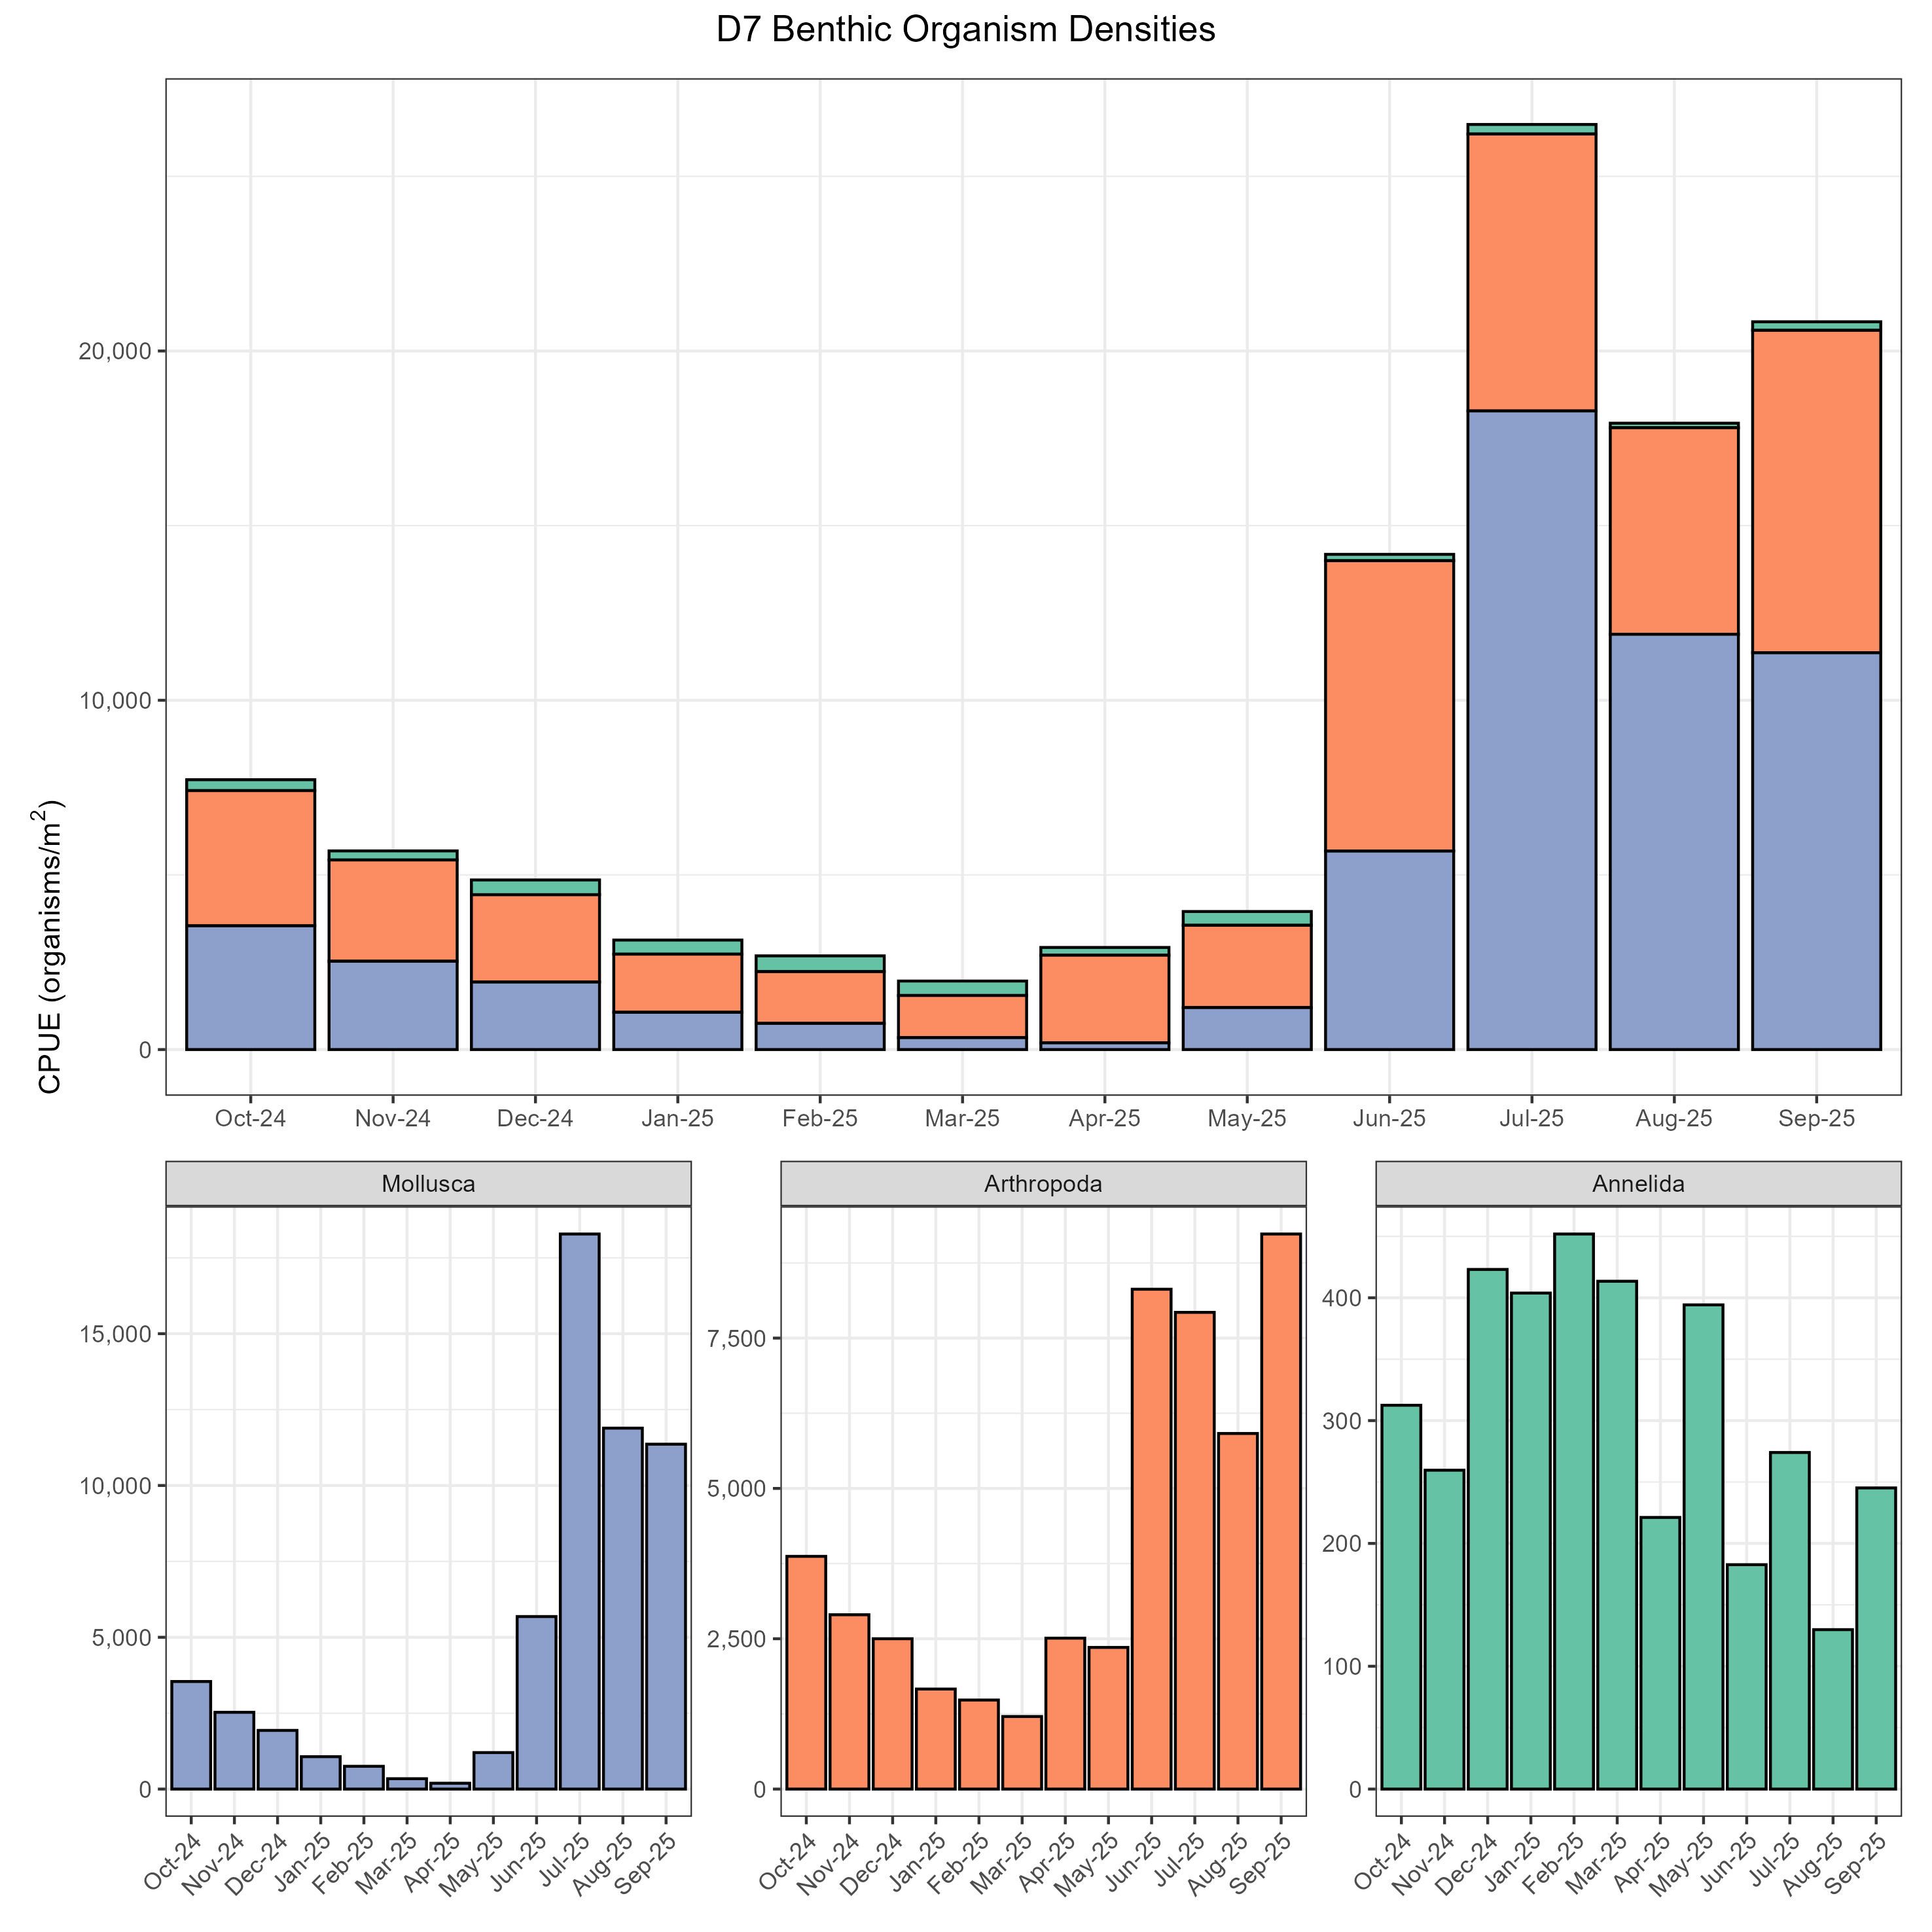
\includegraphics[width=1\linewidth,height=\textheight,keepaspectratio]{admin/figures-tables/benthic/benthic_bar_d7.png}

}

\caption{\label{fig-benthic_d7}Density of benthic organisms, by month,
collected at station D7.}

\end{figure}%

\begin{figure}[H]

\centering{

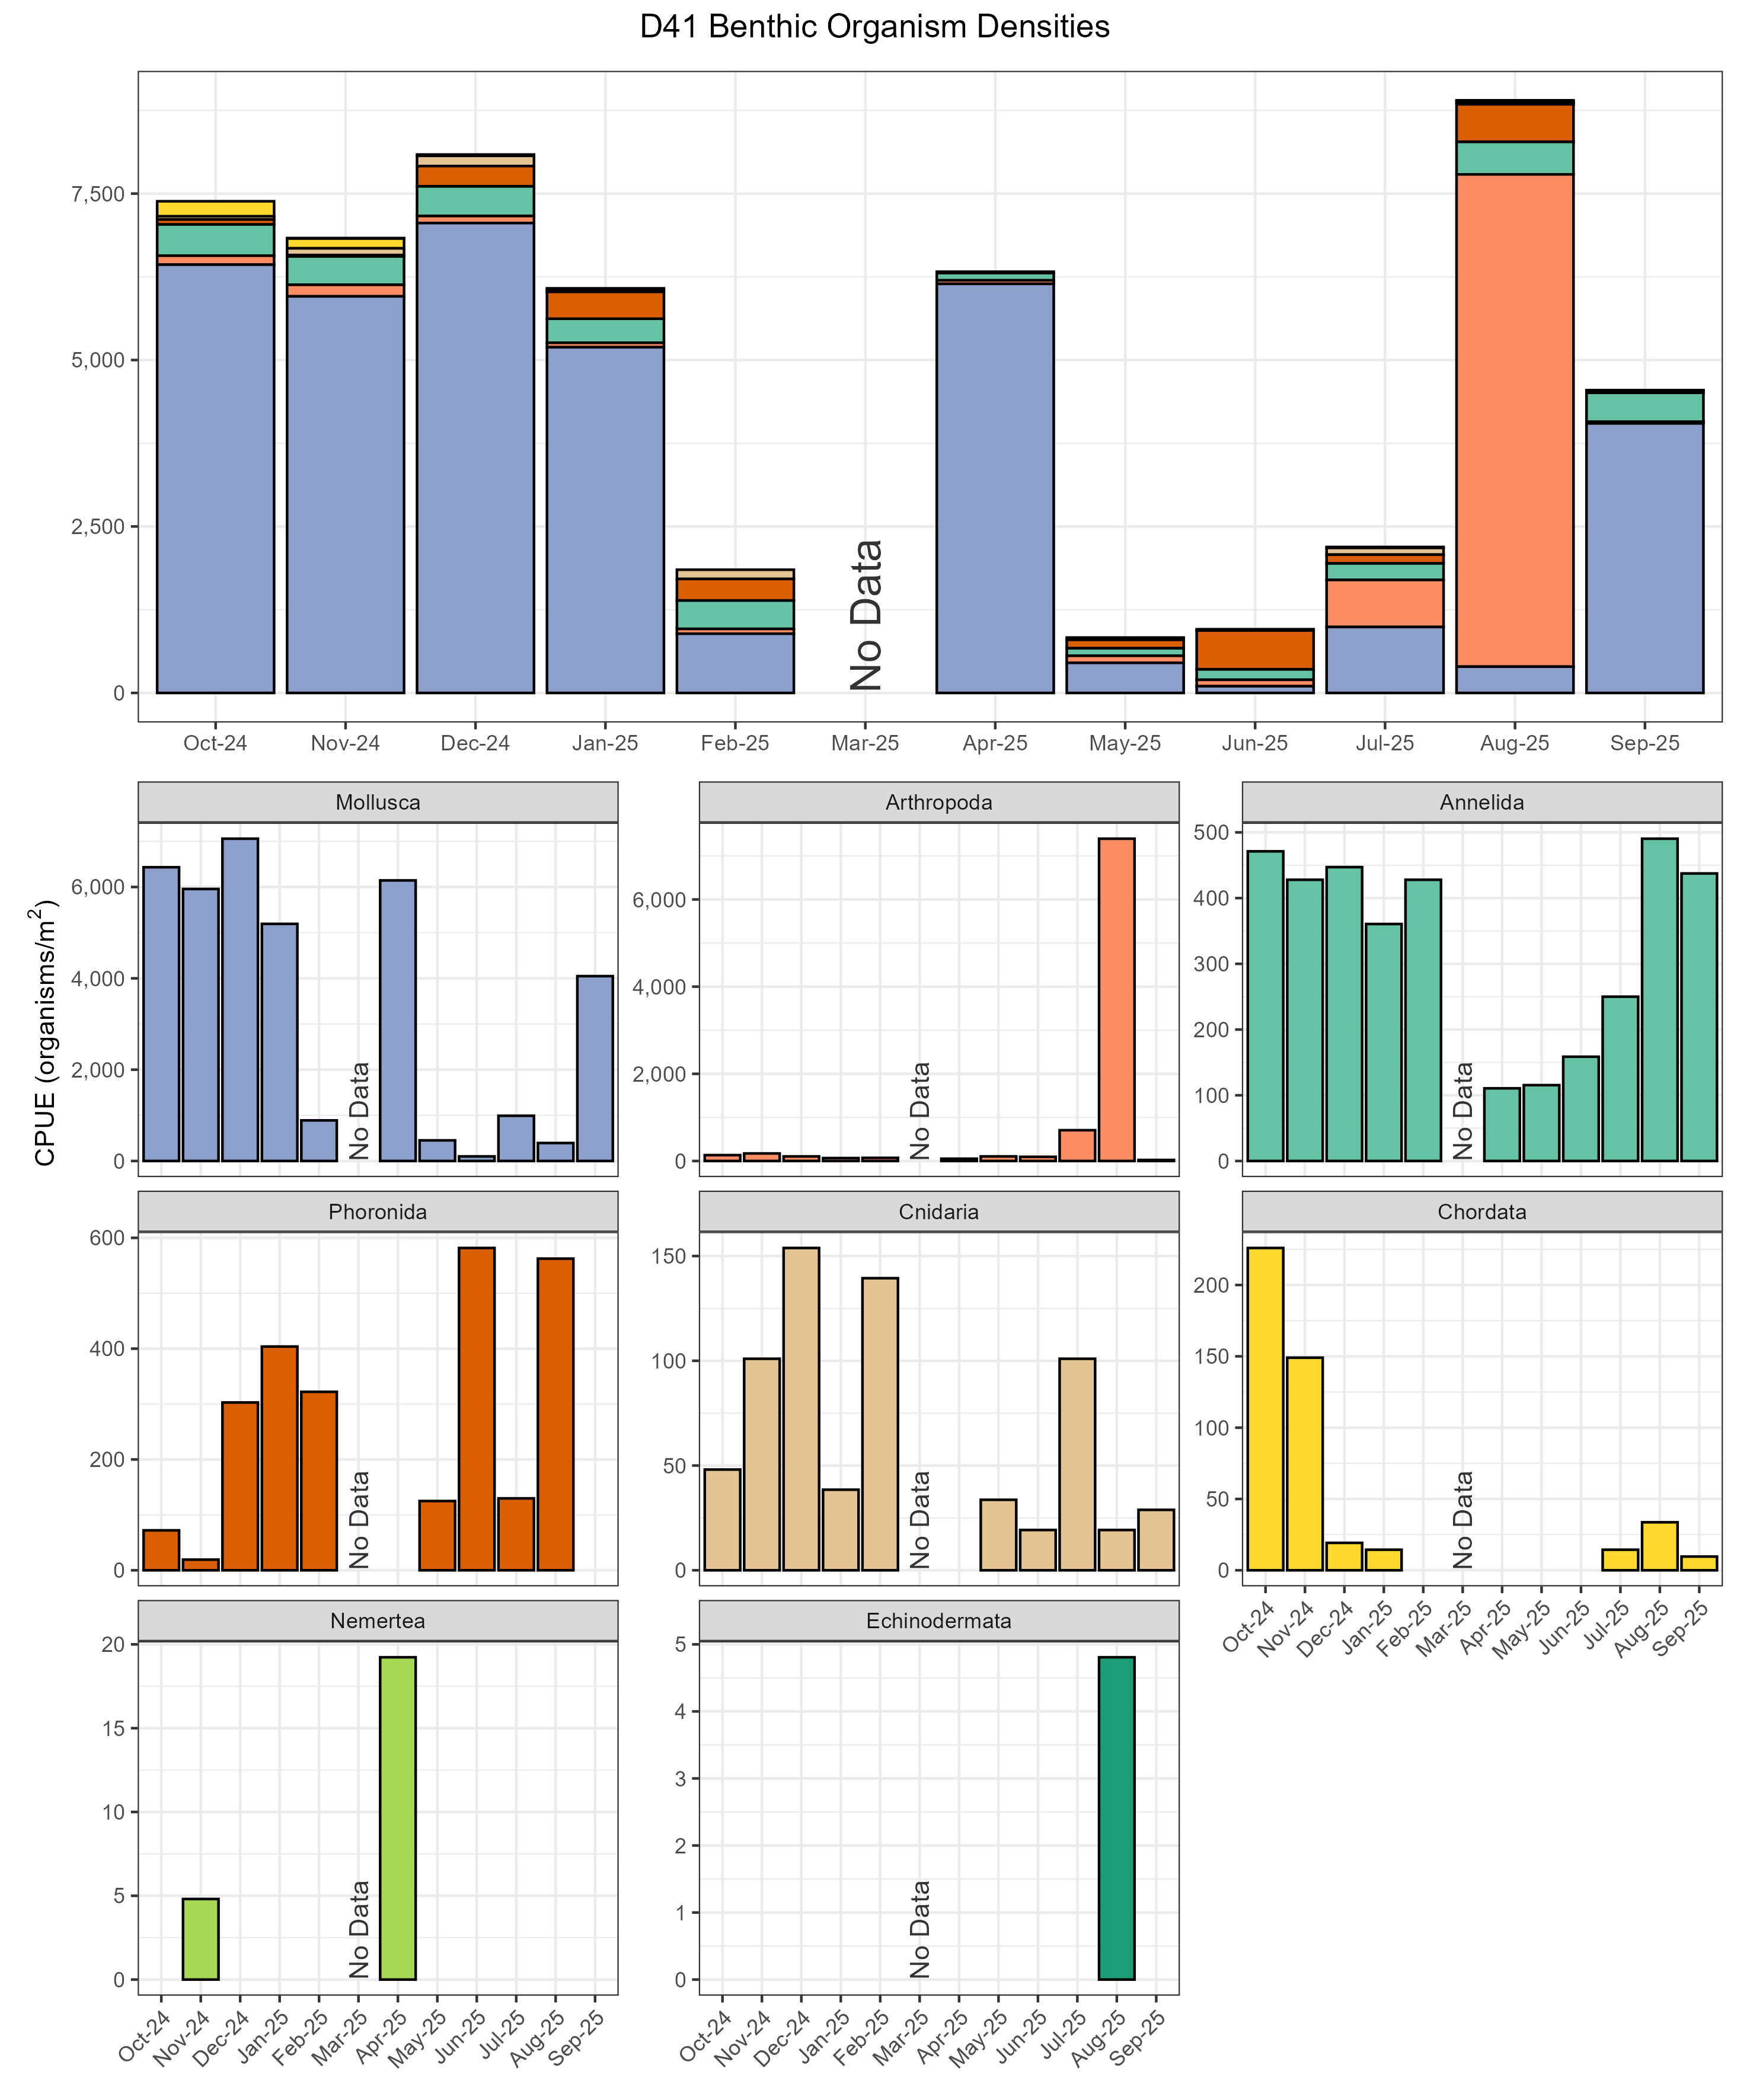
\includegraphics[width=1\linewidth,height=\textheight,keepaspectratio]{admin/figures-tables/benthic/benthic_bar_d41.png}

}

\caption{\label{fig-benthic_d41}Density of benthic organisms, by month,
collected at station D41.}

\end{figure}%

\begin{figure}[H]

\centering{

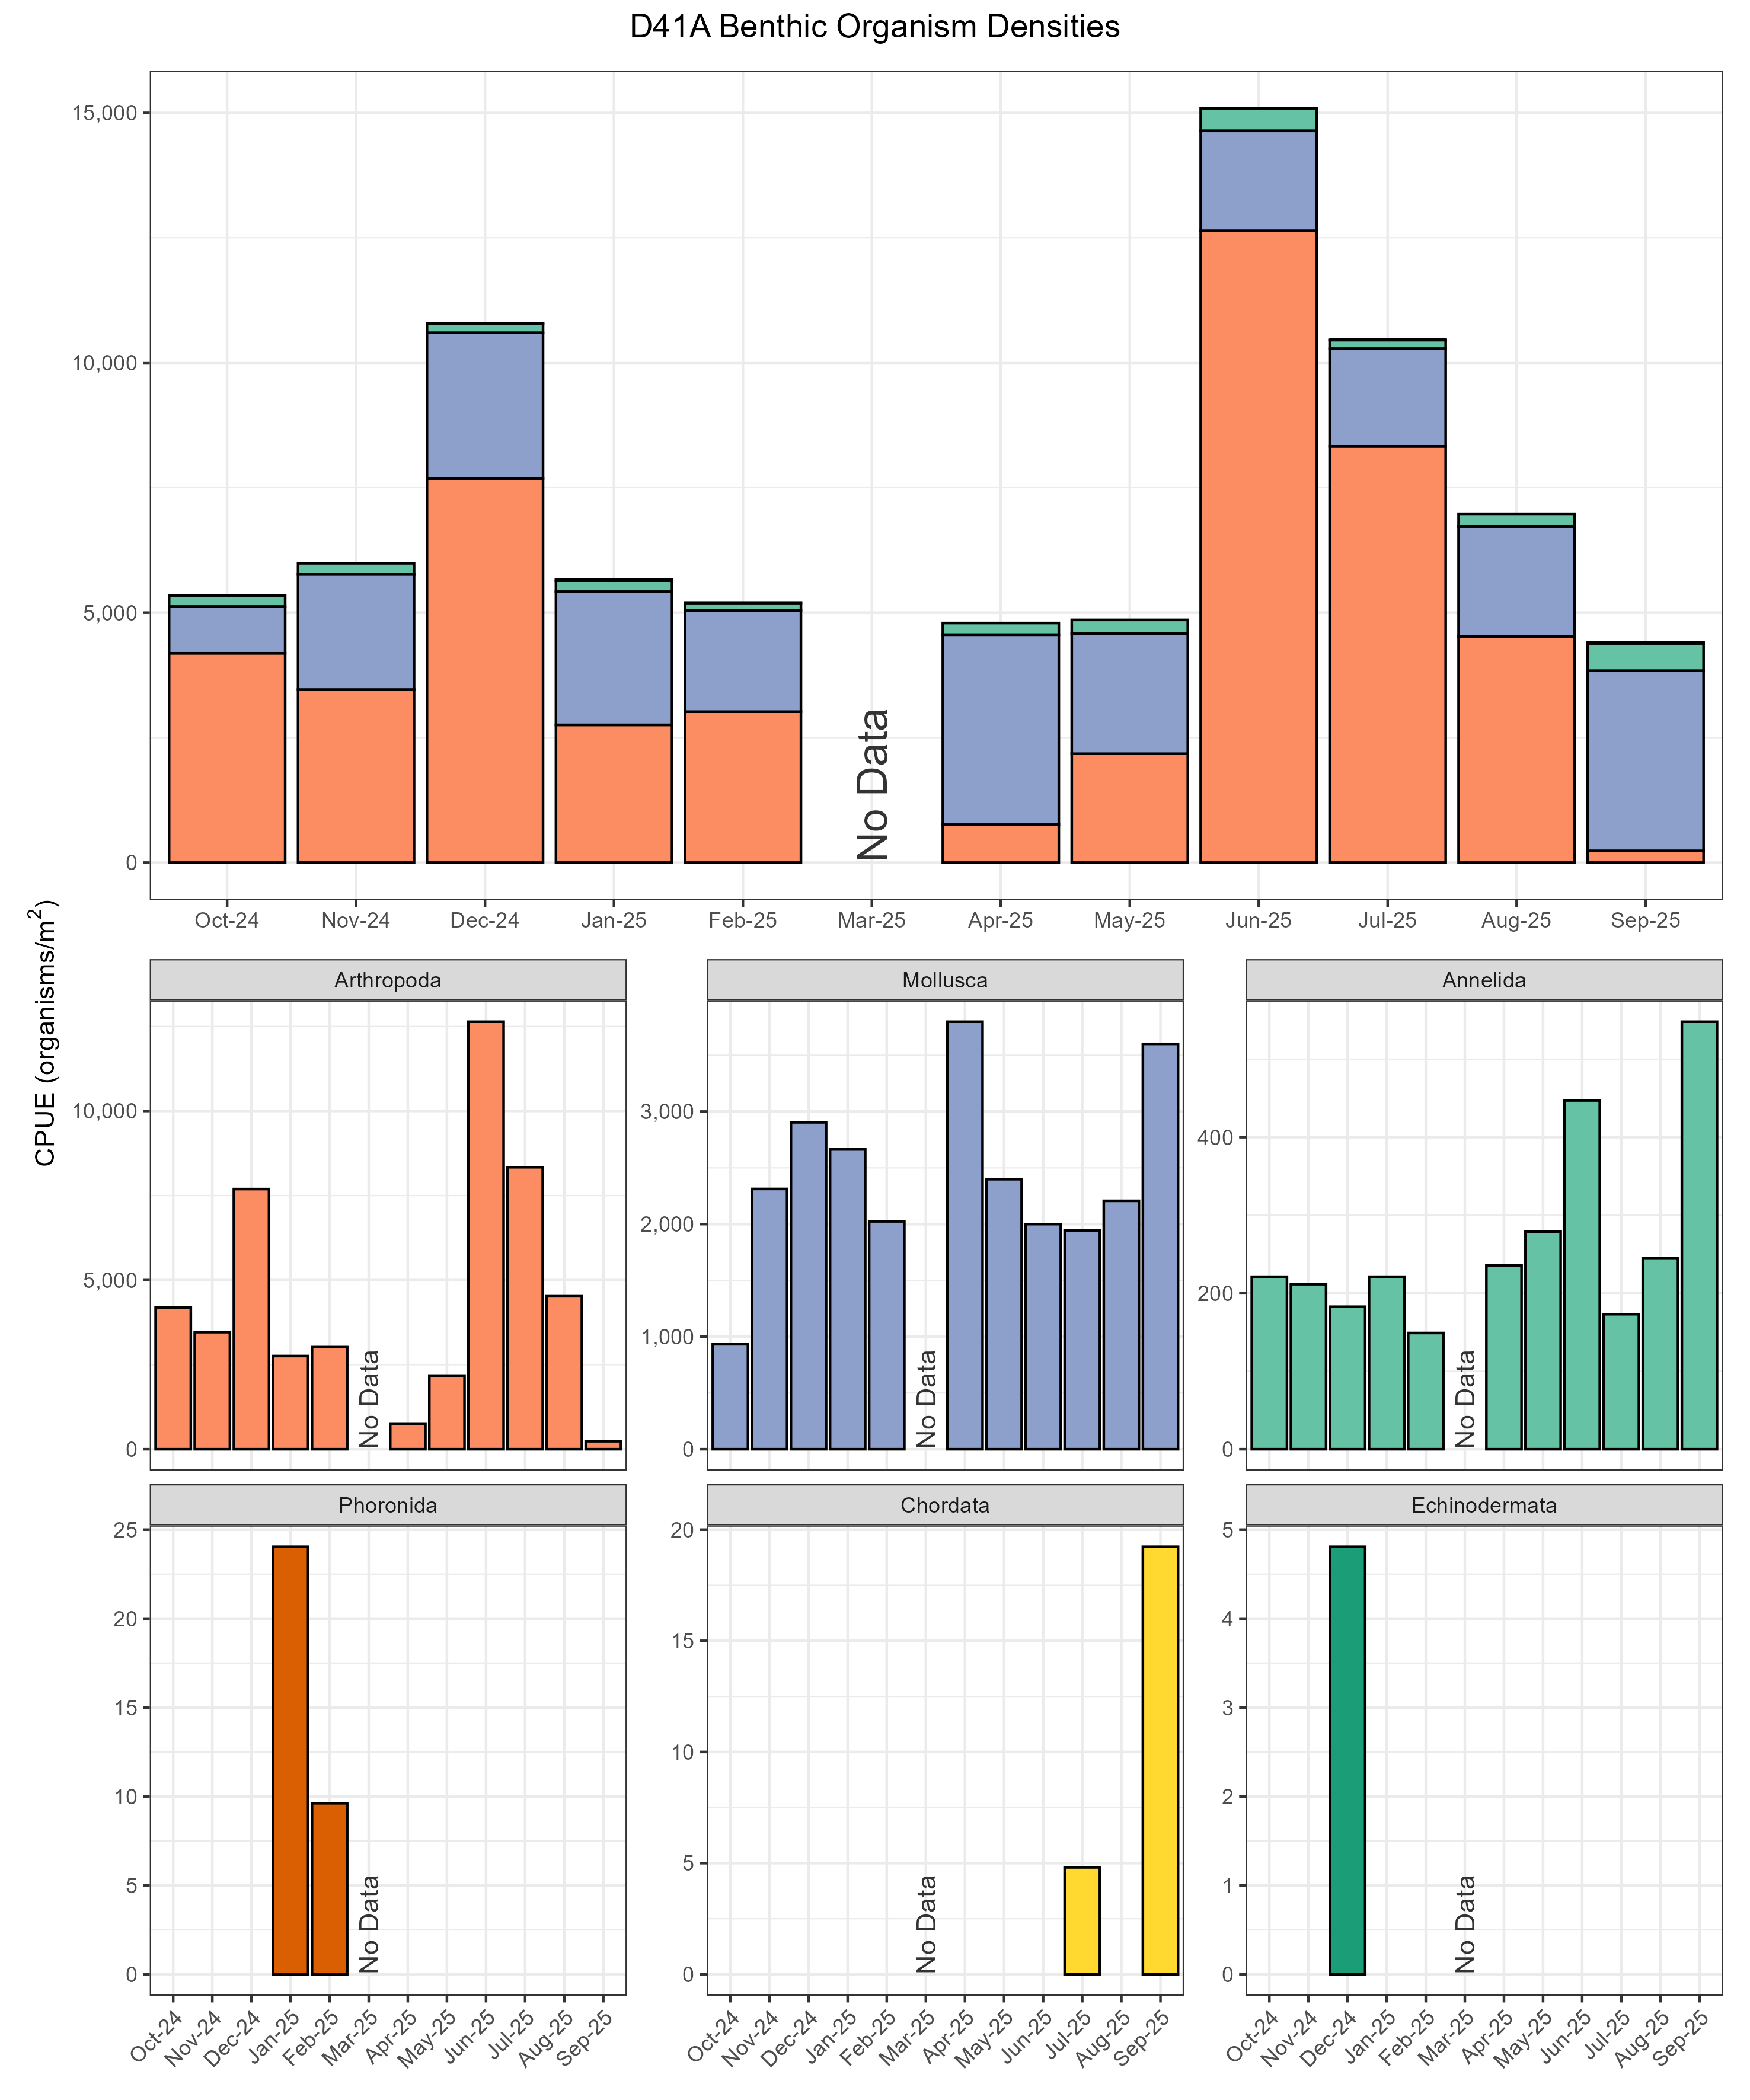
\includegraphics[width=1\linewidth,height=\textheight,keepaspectratio]{admin/figures-tables/benthic/benthic_bar_d41a.png}

}

\caption{\label{fig-benthic_d41a}Density of benthic organisms, by month,
collected at station D41A.}

\end{figure}%

\newpage

\section{Tables}\label{tables}

\begin{table}

\caption{\label{tbl-stations}Stations included within each region of the
Delta}

\centering{

\centering
\begin{tabular}{>{\centering\arraybackslash}p{11.6666666666667em}>{\centering\arraybackslash}p{11.6666666666667em}>{\centering\arraybackslash}p{11.6666666666667em}}
\toprule
Region & WY Index & Stations\\
\midrule
North Delta & Sacramento & D24\\
Central Delta & San Joaquin & D16, D28A\\
South Delta & San Joaquin & C9, P8\\
Confluence & Sacramento & D4\\
Suisun and Grizzly Bays & Sacramento & D6, D7\\
\addlinespace
San Pablo Bay & Sacramento & D41, D41A\\
\bottomrule
\end{tabular}

}

\end{table}%




\end{document}
